\documentclass[compress]{beamer}

\usepackage[nofonts]{ctex}
\setCJKmainfont[ItalicFont={Kaiti SC}]{Kaiti SC}%
%\setCJKmainfont[ItalicFont={AR PL KaitiM GB}]{AR PL KaitiM GB}%
%\setCJKsansfont{WenQuanYi Zen Hei}% 文泉驿的黑体

\mode<beamer>
{
     \useinnertheme{rectangles}
     %\useoutertheme{infolines}
     %\useoutertheme{split}
     \usecolortheme{rose}
     \usecolortheme{seahorse}

     \setbeamertemplate{navigation symbols}{}%remove navigation symbols

     %\expandafter\def\expandafter\insertshorttitle\expandafter{%
     %\insertshorttitle\hfill%
     %\insertframenumber\,/\,\inserttotalframenumber}
    \setbeamertemplate{footline} {
      \leavevmode%
      \hbox{%
      \begin{beamercolorbox}[wd=.1\paperwidth,ht=2.25ex,dp=1ex,left]{date in head/foot}%
        \usebeamerfont{date in head/foot}%
        \hspace*{1ex}\raisebox{-0.8ex}{
\includegraphics[width=3ex]{Overlays/logo.pdf}}%
      \end{beamercolorbox}%
      \begin{beamercolorbox}[wd=.4\paperwidth,ht=2.25ex,dp=1ex,right]{date in head/foot}%
        \usebeamerfont{date in head/foot}\insertsection\hspace*{1ex}
      \end{beamercolorbox}%
      \begin{beamercolorbox}[wd=.4\paperwidth,ht=2.25ex,dp=1ex,left]{date in head/foot}%
        \usebeamerfont{date in head/foot}\hspace*{1ex}\insertsubsection
      \end{beamercolorbox}%
      \begin{beamercolorbox}[wd=.1\paperwidth,ht=2.25ex,dp=1ex,right]{date in head/foot}%
        \insertframenumber{} / \inserttotalframenumber\hspace*{1ex}
      \end{beamercolorbox}}%
      \vskip0pt%
    }
}

%\defbeamertemplate*{footline}{mytheme}
%{
%  \leavevmode%
%  \hbox{%
%  \begin{beamercolorbox}[wd=.4\paperwidth,ht=2.25ex,dp=1ex,center]{author in head/foot}%
%    \usebeamerfont{author in head/foot}\insertshortauthor
%  \end{beamercolorbox}%
%  \begin{beamercolorbox}[wd=.2\paperwidth,ht=2.25ex,dp=1ex,center]{institute in head/foot}%
%    \usebeamerfont{institute in
%    head/foot}\insertshortinstitute\hspace*{2em}%
%    \raisebox{-1ex}{
\includegraphics[width=3ex]{Overlays/logo.pdf}}%
%  \end{beamercolorbox}%
%  \begin{beamercolorbox}[wd=.4\paperwidth,ht=2.25ex,dp=1ex,right]{title in head/foot}%
%    \usebeamerfont{title in head/foot}\insertshorttitle{}\hspace*{2em}
%    \insertframenumber{} / \inserttotalframenumber\hspace*{2ex} 
%  \end{beamercolorbox}}%
%  \vskip0pt%
%}
%\usebeamertemplate{mytheme}

\mode<handout>
{
	\usetheme{default}
	\usepackage{pgfpages}
	\pgfpagesuselayout{2 on 1}[a4paper,landscape,border shrink=5mm]
}


\usepackage{amsmath,latexsym,amssymb,amsfonts,amsbsy}
\usepackage{graphicx}
\usepackage{array}
\usepackage{hyperref}
\usepackage{textpos}
\usepackage{ulem}
\usepackage{comment}
\usepackage{fancyvrb}
\fvset{frame=single, numbers=left, fontsize=\small}
\usepackage{tikz}
\usetikzlibrary{calc,arrows.meta, graphs, trees, shapes, positioning, decorations.markings, intersections, decorations.text}
\usepackage{tikz-uml}

\newcommand{\romannumber}[1]{{\textrm{\uppercase\expandafter{\romannumeral
#1}}}}

\graphicspath{{figure/}}

%%%%%%%%%%%%%%%%%%%%%%%%%%%%%%%%%%%%%%%%%%%%%%%%%%%%%%%%%%%%%%%%%
%    body                                                       %
%%%%%%%%%%%%%%%%%%%%%%%%%%%%%%%%%%%%%%%%%%%%%%%%%%%%%%%%%%%%%%%%%


\begin{document}

\AtBeginSection[]
{ 
    \begin{frame}<beamer> 
		\frametitle{内容提要} 
		\tableofcontents[currentsection,currentsubsection,
        subsectionstyle=show/shaded/hide] 
	\end{frame} 
} 

					
\title{第八章 ~~  面向对象的系统设计\MakeUppercase{\romannumeral 2}}

\author[面向对象的分析与设计]
{曹东刚\\\href{mailto:caodg@pku.edu.cn}{caodg@pku.edu.cn}}

\institute[北京大学]{北京大学信息学院研究生课程 - 面向对象的分析与设计 \\
    \href{http://sei.pku.edu.cn/~caodg/course/oo}{http://sei.pku.edu.cn/\~{}caodg/course/oo}}

\date{}

\titlegraphic{
\includegraphics[height=0.10\textwidth]{Overlays/logo.pdf}}

\begin{frame}[plain]
	\titlepage
\end{frame}

\setcounter{framenumber}{0}

\section{控制驱动部分的设计}

\subsection[背景]{背景及相关技术介绍}

\begin{frame}
  \frametitle{什么是控制驱动部分}
  \begin{block}{控制驱动部分}
    是OOD模型的外围组成部分之一,由系统中全体\uline{主动类}构成。这些
    主动类描述了整个系统中所有的\uline{主动对象},每个主动对象是系统中一
    个\uline{控制流}的驱动者 
  \end{block}

  控制流(control flow):\uline{进程}(process)和\uline{线程}(thread)的总称 \\

  有多个控制流并发执行的系统称作\uline{并发系统}(多任务系统)

\end{frame}

\begin{frame}
  \frametitle{为什么需要控制驱动部分}
  \begin{itemize}
    \item 并发行为是现实中固有的
      \begin{itemize}
        \item 外围设备与主机并发工作的系统
        \item 有多个窗口进行人机交互的系统
        \item 多用户系统
        \item 多个子系统并发工作的系统
        \item 单处理机上的多任务系统
        \item 多处理机系统
      \end{itemize}

    \item 多任务的设置
      \begin{itemize}
        \item 描述问题域固有的并发行为
        \item 表达实现所需的设计决策
      \end{itemize}

    \item 隔离硬件、操作系统、网络的变化对整个系统的影响
  \end{itemize}
\end{frame}


\begin{frame}
  \frametitle{由系统总体方案决定的实现条件}
  \begin{itemize}
    \item 计算机硬件:性能、容量和CPU数目
    \item 操作系统:对并发和通讯的支持
    \item 网络方案:网络软硬件设施、网络拓扑结构、通讯速率、网络协议等
    \item 软件体系结构
    \item 编程语言:对进程和线程的描述能力
    \item 其它软件:如数据管理系统、界面支持系统、构件库等
  ——对共享和并发访问的支持
  \end{itemize}
\end{frame}

\begin{frame}
  \frametitle{软件体系结构}
  \begin{block}{软件体系结构}
    描述了构成系统的元素、这些元素之间的相互作用、指导其组合的
  模式以及对这些模式的约束
\end{block}
几种典型的软件体系结构风格
\begin{itemize}
  \item 管道与过滤器风格(pipe and filter style)
  \item 面向对象风格(object-oriented style)
  \item 层次风格(layered style)
  \item 黑板风格(blackboard style)
  \item 进程控制风格(process control style)
  \item 客户-服务器风格(client-server style) 
\end{itemize}

\end{frame}

\begin{frame}
  \frametitle{分布式系统的体系结构风格}
  \begin{itemize}
    \item 主机+仿真终端体系结构
    \item 文件共享体系结构
    \item 客户-服务器体系结构
      \begin{itemize}
        \item 二层客户-服务器体系结构
        \item 三层客户-服务器体系结构
        \item 对等式客户-服务器体系结构
        \item 瘦客户-服务器体系结构
        \item 胖客户-服务器体系结构
      \end{itemize}
    \item 浏览器-服务器体系结构
  \end{itemize}

\end{frame}

\begin{frame}
  \frametitle{系统的并发性}
  \only<1> {
    进程(process)概念出现之前,并发程序设计困难重重,
    主要原因:
    \begin{itemize}
      \item 并发行为彼此交织,理不出头绪
      \item 与时间有关的错误不可重现
    \end{itemize}

    \uline{进程}概念的提出使这个问题得到根本解决
  }

  \only<2> {
    进程的全称是\uline{顺序进程}(sequential process),其基本思想是把并发程序分
    解成一些顺序执行的进程,使得:

    \begin{itemize}
      \item 每个进程内部不再包含并发行为 \\
    \quad 所以叫做顺序进程,其设计避免了并发问题
      \item 多个进程之间是并发(异步)执行的 \\
    \quad 所以能够构成并发程序
    \end{itemize}
  }
\end{frame}

\begin{frame}
  \frametitle{进程与线程}
  由于并行计算的需要,要求人为地在\uline{顺序程序内部}定义和识别可
  \uline{并发执行}的单位
  ,线程的概念就诞生了 \\[2ex]

  \textcolor{blue}{线程与进程的区别}:

  \begin{itemize}
    \item 进程既是处理机分配单位,也是存储空间、设备等资源的分配单位(重量级的控
  制流)

\item 线程只是处理机分配单位(轻量级的控制流) 

\item 一个进程可以包含多个线程,也可以是单线程的
  \end{itemize}
\end{frame}

\begin{frame}
  \frametitle{应用系统的并发性}
  \only<1> {
  \textcolor{blue}{ 从网络、硬件平台的角度看}:
  \begin{itemize}
    \item 分布在不同计算机上的进程之间的并发
    \item 在多CPU的计算机上运行的进程或线程之间的并发
    \item 在一个CPU上运行的多个进程或线程之间的并发
  \end{itemize}
}

\only<2> {
  \textcolor{blue}{从应用系统的需求看}:
  \begin{itemize}
    \item 需要跨地域进行业务处理的系统
    \item 需要同时使用多台计算机或多个CPU进行处理的系统
    \item 需要同时供多个用户或操作者使用的系统
    \item 需要在同一时间执行多项功能的系统
    \item 需要与系统外部多个参与者同时进行交互的系统
  \end{itemize}
}
\end{frame}

\begin{frame}
  \frametitle{处理应用系统并发的例子}

  \label{app:satallite}
  \only<1> {
    \textbf{问题描述:} \\[2ex]
    某单位想开发一个卫星遥感信息处理系统,要求是:实时把通过地面接收设备
    传来的卫星遥感图片信息\uline{输入系统},经过必要的\uline{数据处理},
    及时将图片\uline{显示在屏幕上}。
  }

  \only<2> {
  \centering\begin{figure}
  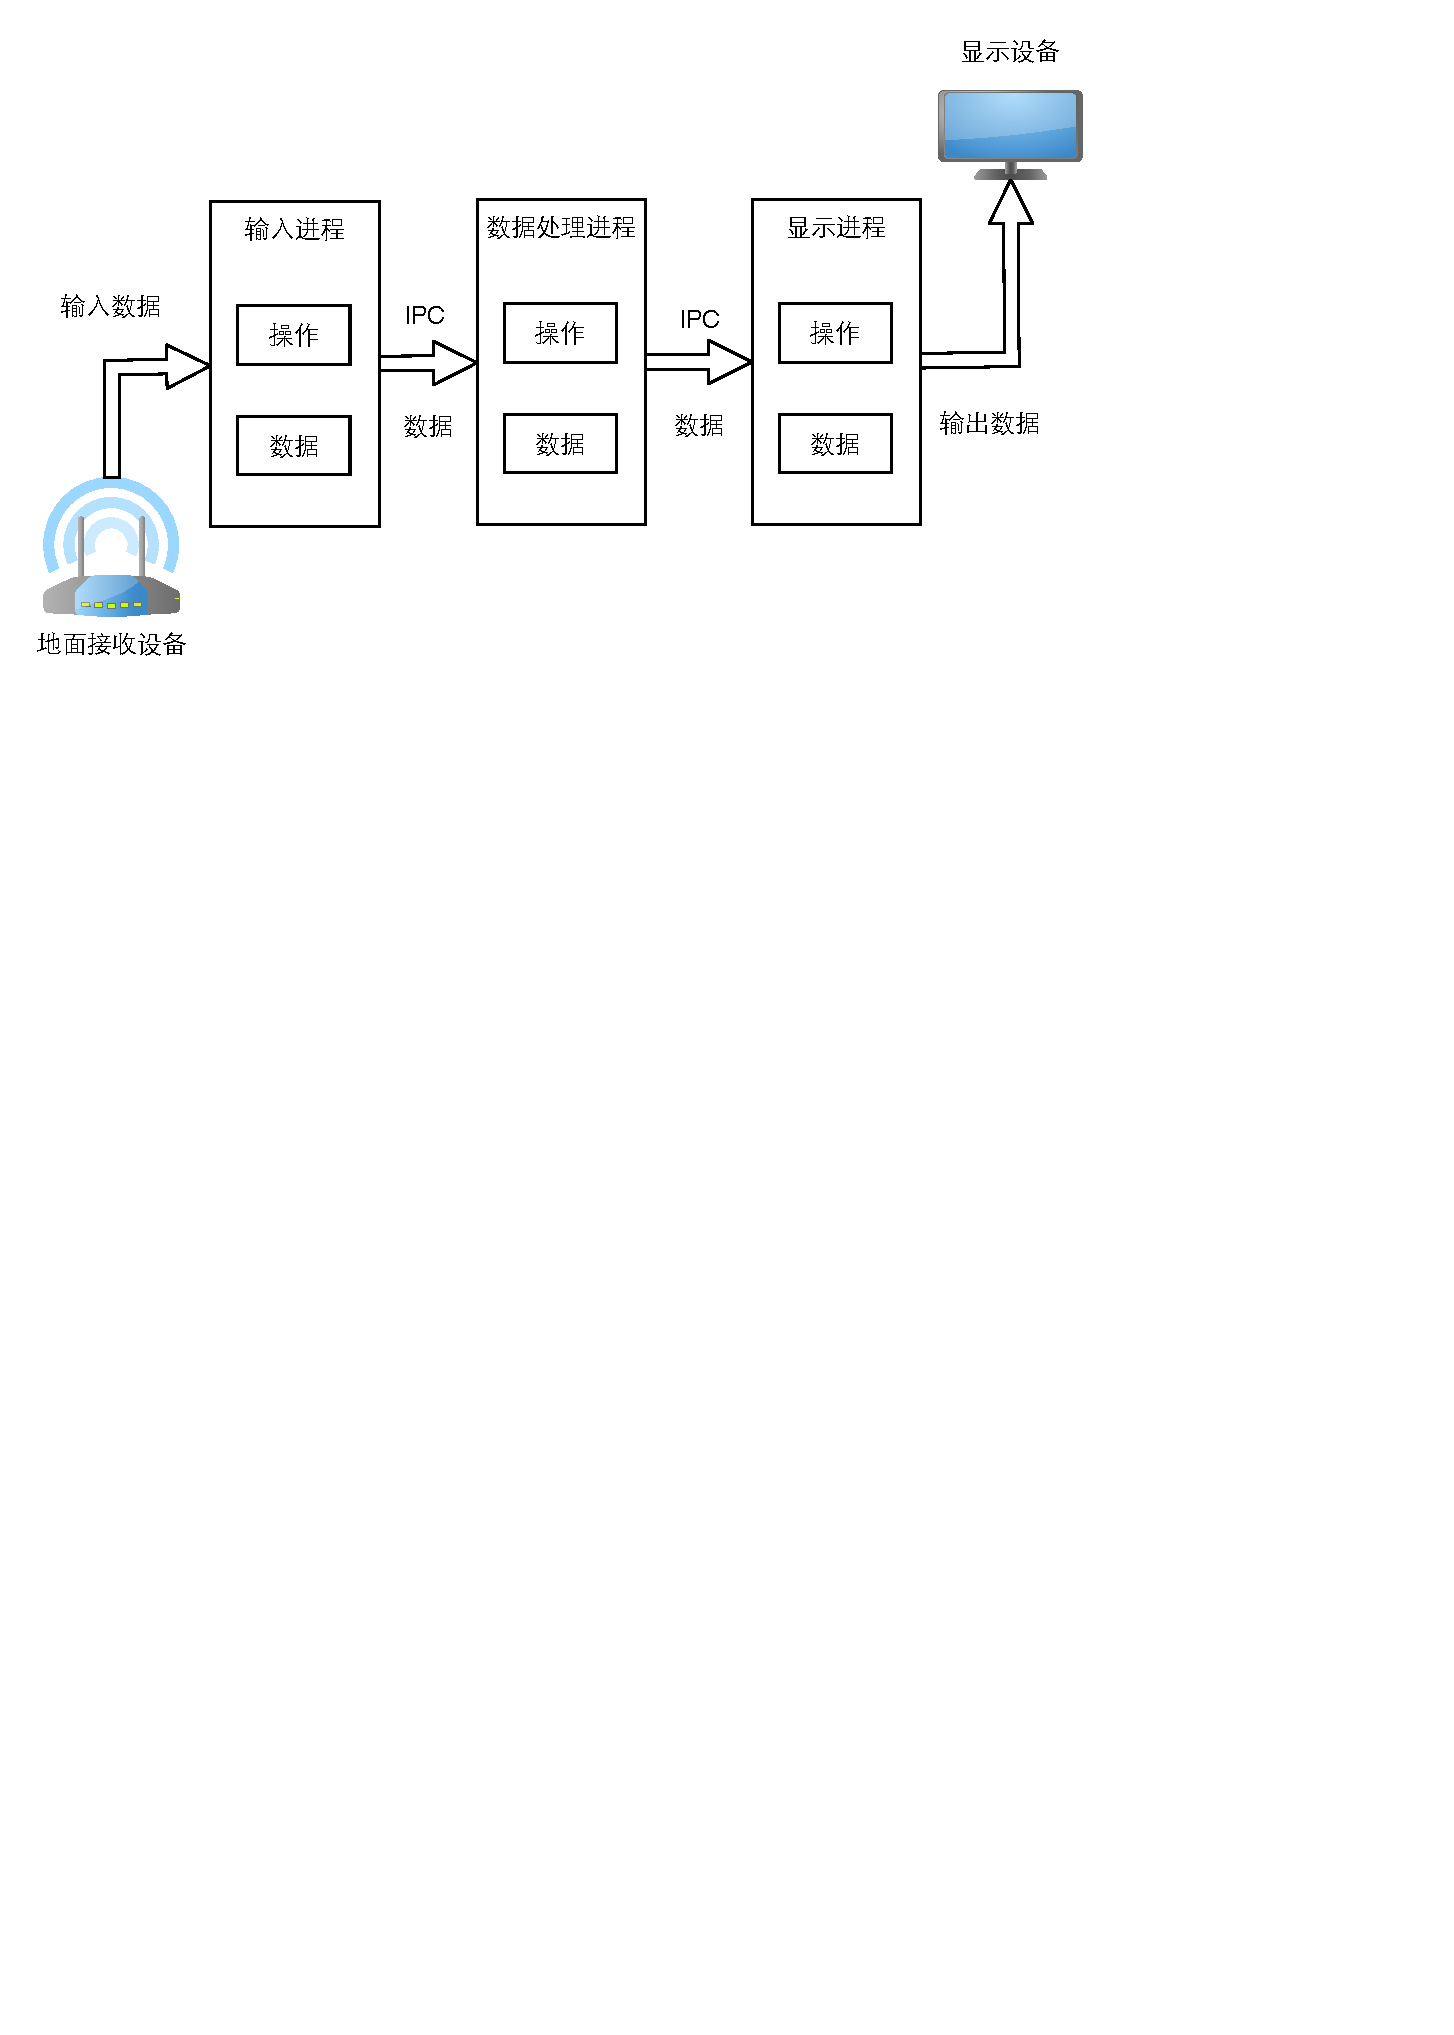
\includegraphics[width=0.9\hsize]{yaogan-processes.pdf}

  用多进程实现的遥感信息处理系统
  \end{figure}
  }

  \only<3> {
    \textbf{新的需求:} \\[2ex]
    针对前页\ref{app:satallite}例子中多进程共享数据速度慢的问题,希望改
    变设计,采用\uline{多线程技术}实现并发,避免控制流之间传送大量数据。
  }
  \only<4> {
  \centering\begin{figure}
  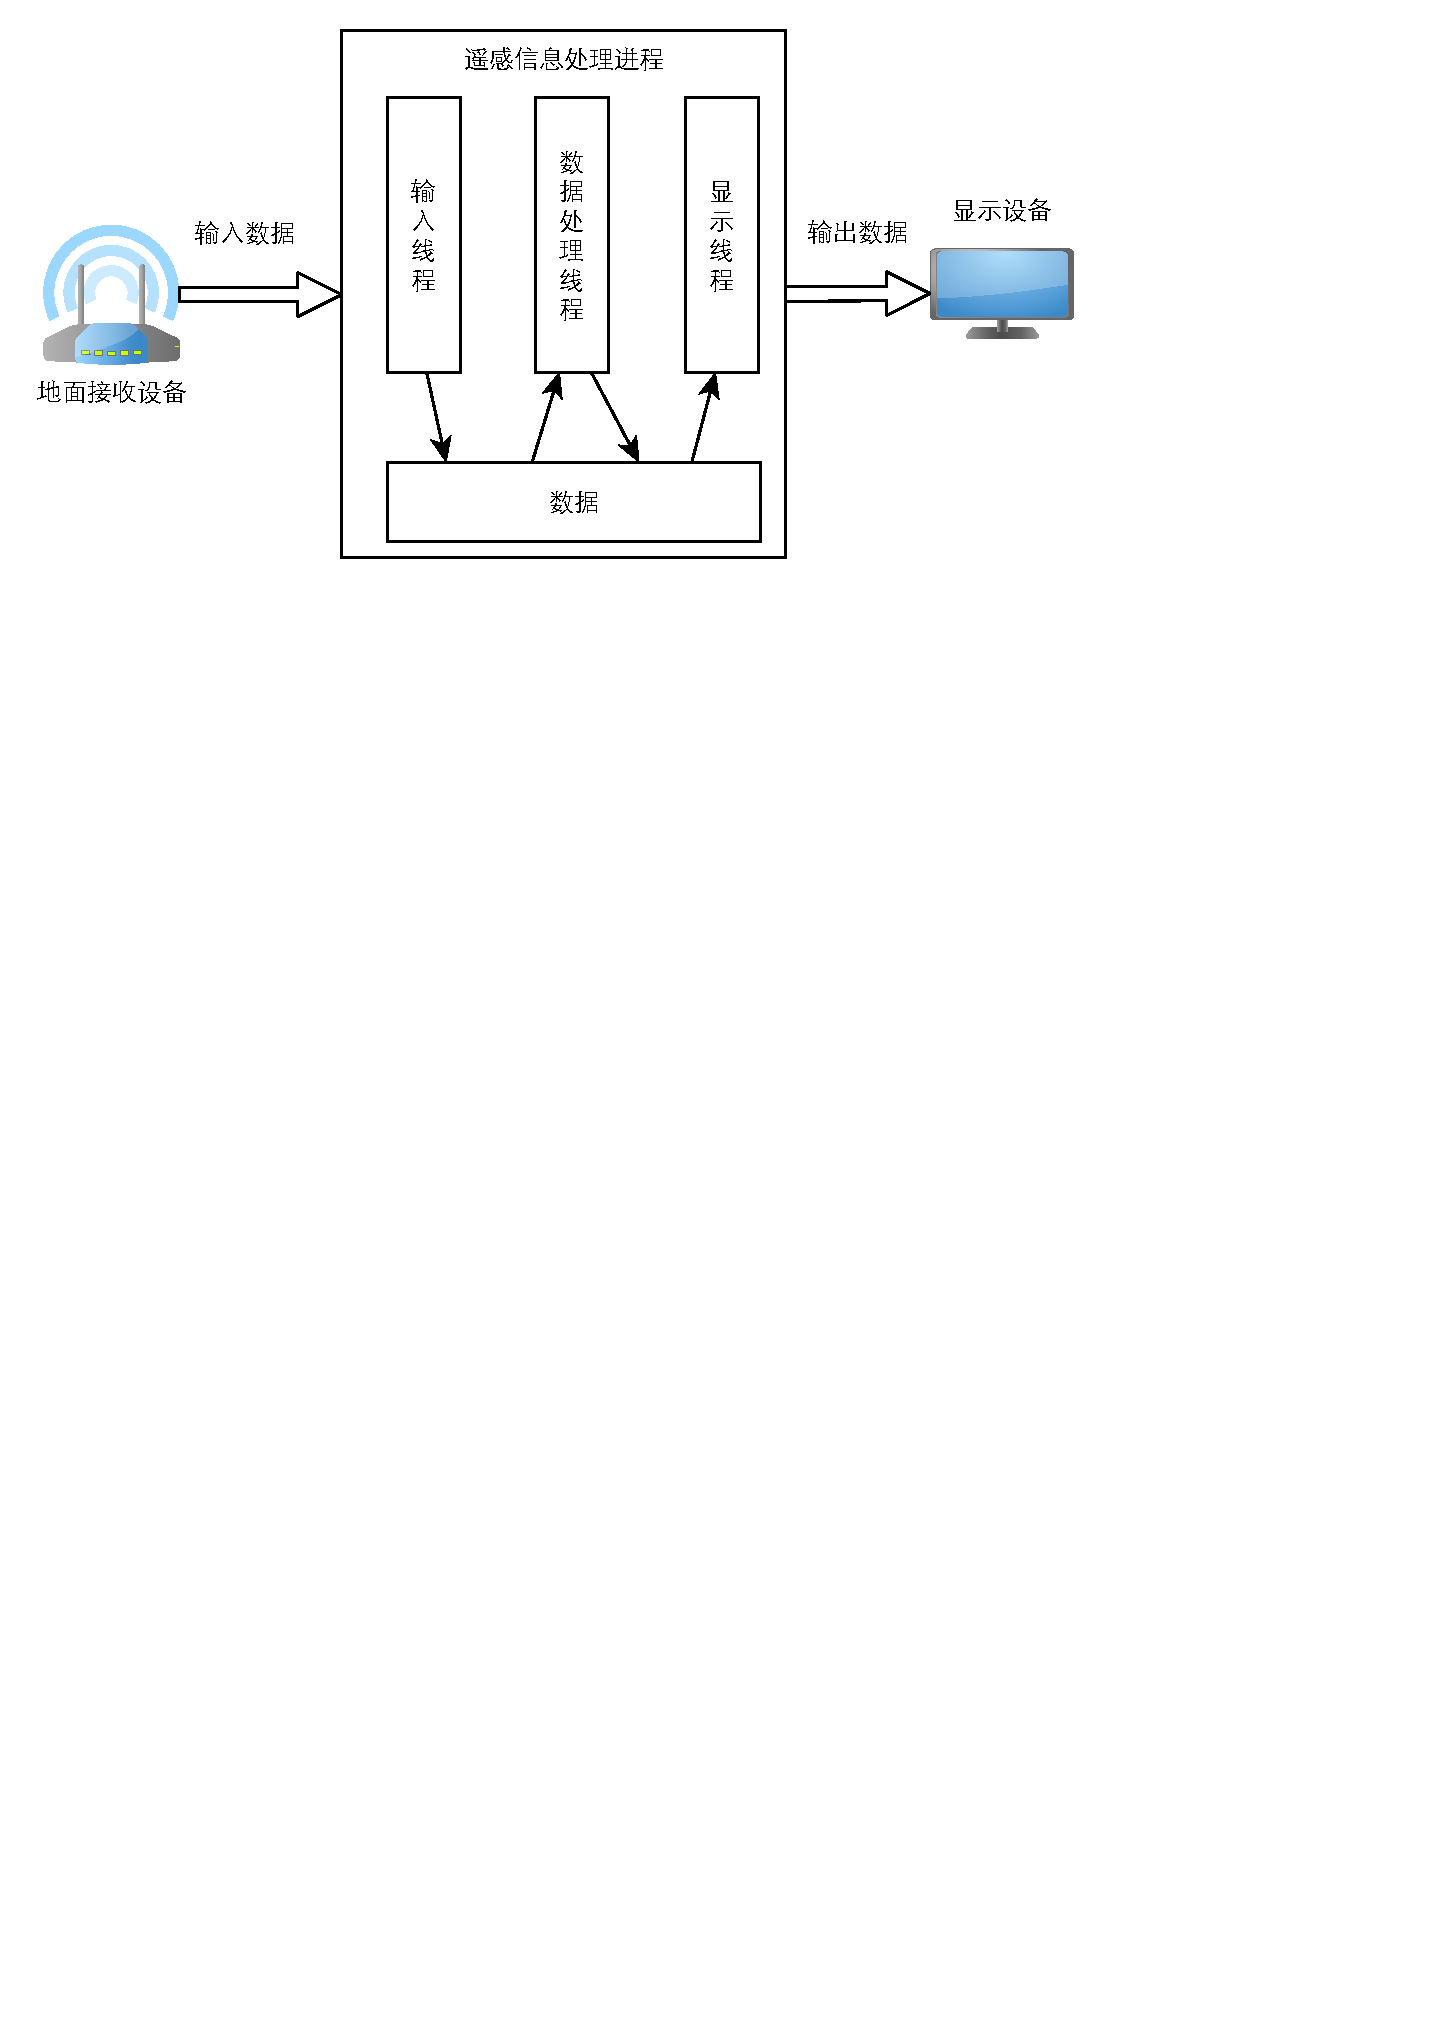
\includegraphics[width=0.9\hsize]{yaogan-threads.pdf}

  用多线程实现的遥感信息处理系统
  \end{figure}
  }

  \only<5> {
    \textbf{拓展业务:} \\[2ex]
    考虑面向不同应用的遥感信息处理系统,不仅需要把图片信息实时显示出来,
    而且需进行\uline{更多处理},如面向地理信息系统的特征信息提取等。
  }
  \only<6> {
  \centering\begin{figure}
  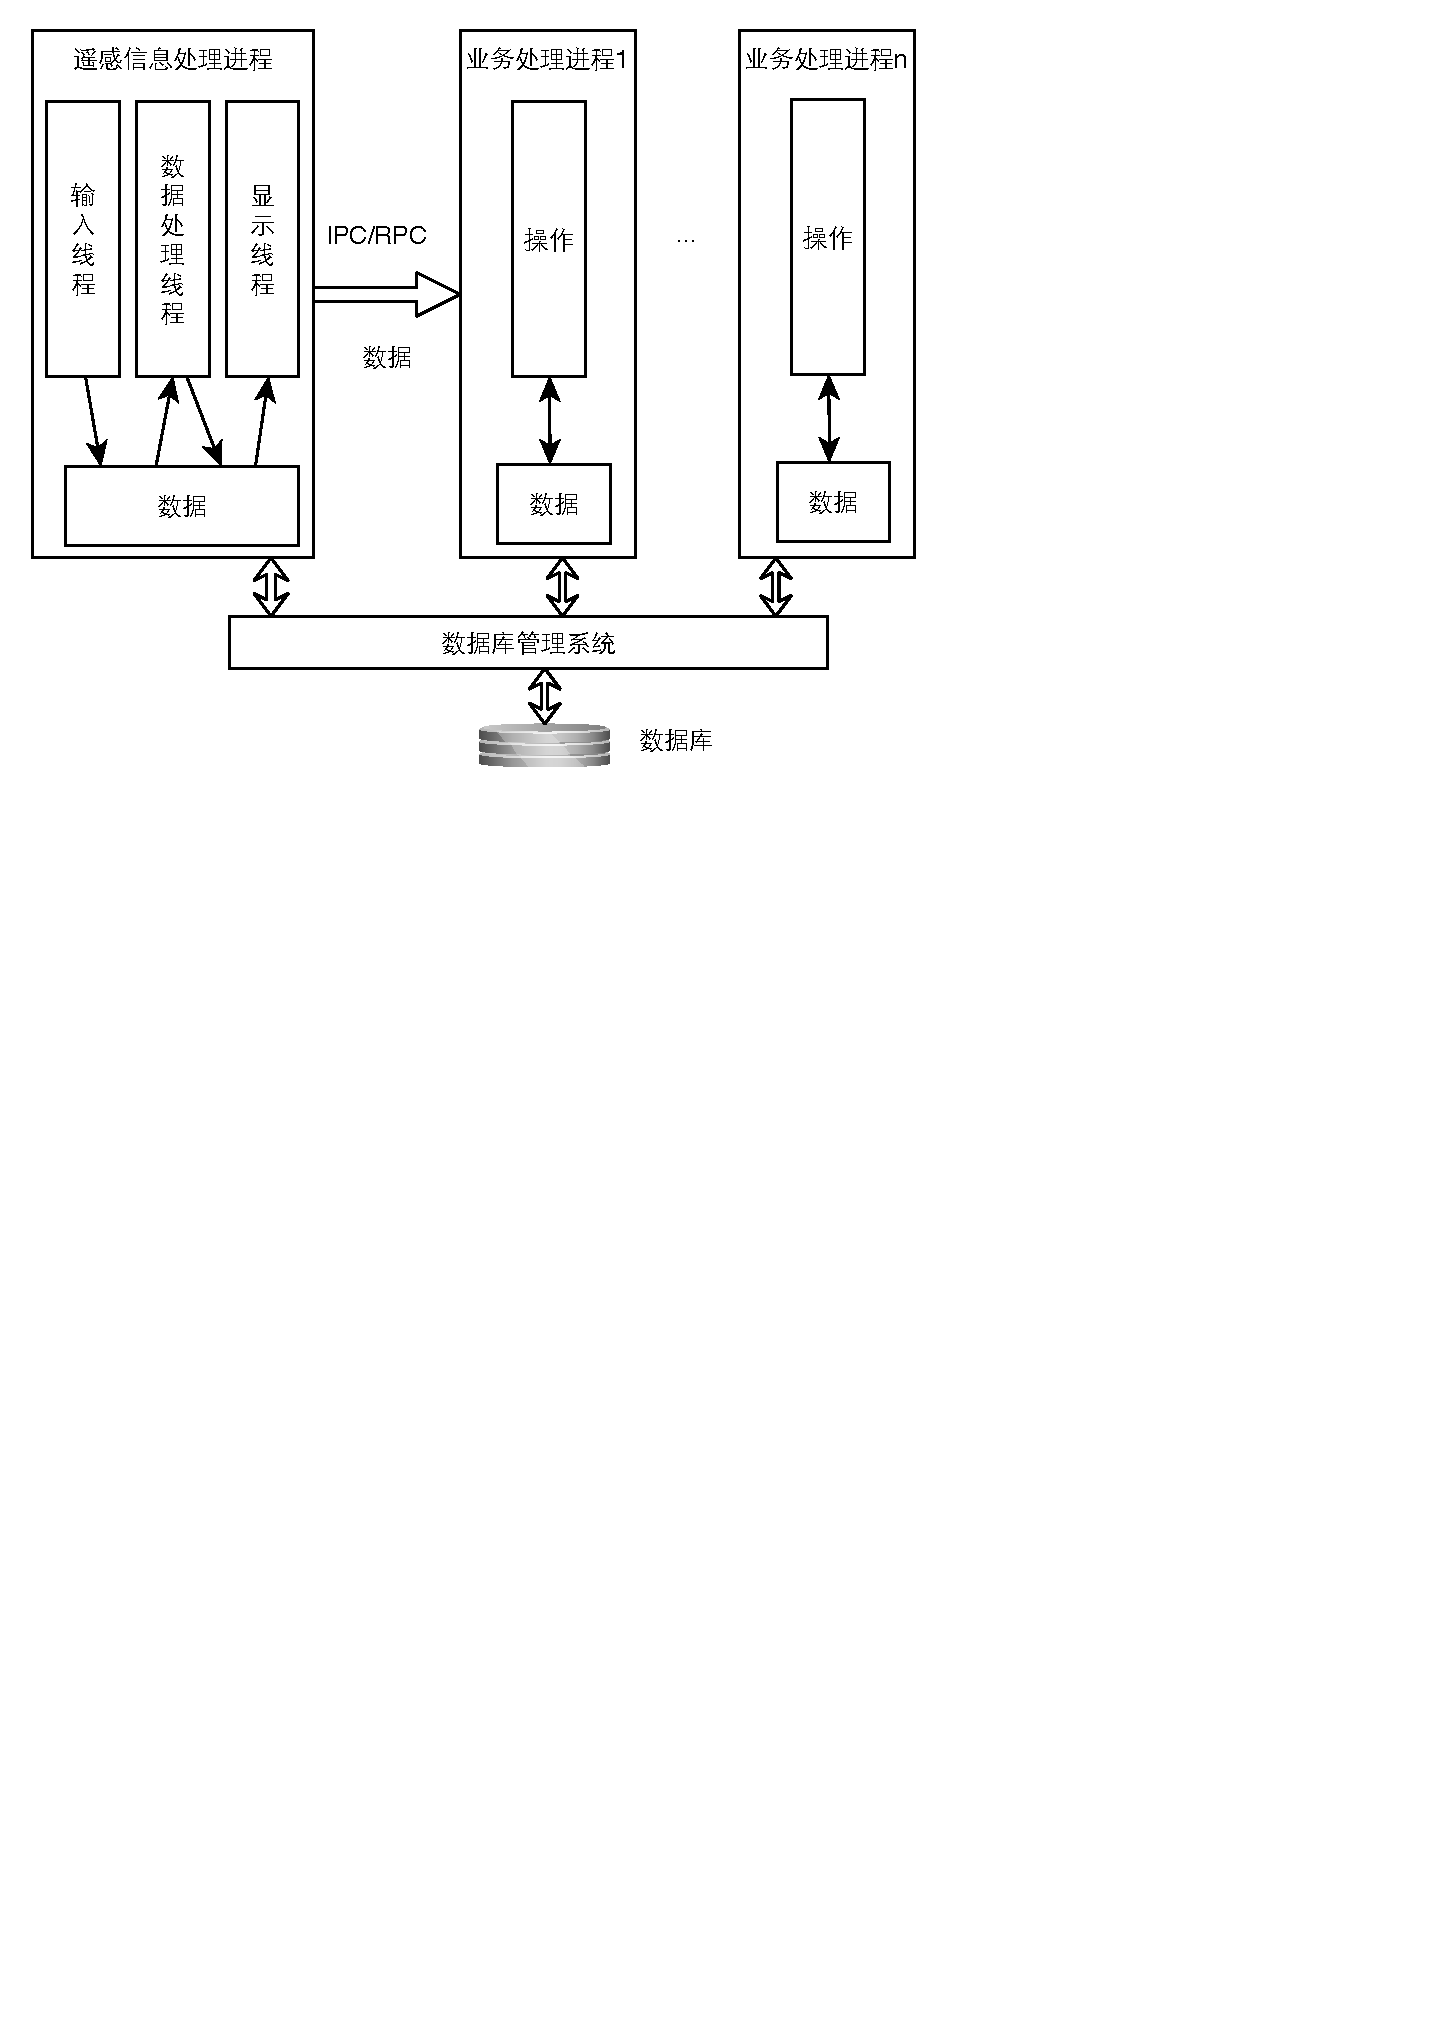
\includegraphics[width=0.8\hsize]{yaogan-mix.pdf}

  同时采用多线程和多进程的多应用遥感信息处理系统
  \end{figure}
  }
\end{frame}

\begin{frame}
  \frametitle{讨论:进程 vs 线程}
  \fbox{
    \parbox{0.8\hsize} {
    \textbf{进程}:重量,分布内存 \\
    \textbf{线程}:轻量,共享内存
    }
  } \\[2ex]

  \begin{itemize}
    \item 数据访问的成本和效率?
    \item 创建、销毁、切换的代价?
    \item 健壮性?
    \item 易于程序员编写并发程序?
  \end{itemize}
\end{frame}

\subsection[如何设计]{如何设计控制驱动部分}

\begin{frame}
  \frametitle{选择软件体系结构风格}

  \begin{itemize}
    \item 二层客户--服务器体系结构 \\
    (数据)服务器--客户机
    \item 三层客户--服务器体系结构 \\
    数据服务器--应用服务器--客户机 
    \item 浏览器--服务器体系结构
  \end{itemize}
\end{frame}

\begin{frame}
  \frametitle{确定系统分布方案}

  \only<1> {
  \fbox{
    \parbox{0.8\hsize}{
      考虑分布方案\uline{之前}:\uline{暂时}将系统看作\uline{集中式}的 \\
      确定分布方案\uline{之后}:将对象分布到各个处理机上, \\
以\textcolor{blue}{每台处理机上的类作为一个包}
   }
 } \\[2ex]

  \begin{tikzpicture}
    \tikzumlset{fill package=white}
    \node [rectangle, draw, align=center,  
      minimum width=1.5cm, minimum height=3cm] {集中式 \\类图} ;
    \draw [->, line width=2pt, >=stealth] (1.2, 0) -- ( 2.2, 0) ; 
    \draw [->, line width=2pt, >=stealth] (1.2, 0.5) -- ( 2.2, 1) ; 
    \draw [->, line width=2pt, >=stealth] (1.2, -0.5) -- ( 2.2, -1) ; 
    \begin{umlpackage}[x=3.5, y=1.5]{A}
    \end{umlpackage}
    \begin{umlpackage}[x=3.5, y=-1.5]{B}
    \end{umlpackage}
    \begin{umlpackage}[x=6.5]{C}
    \end{umlpackage}
    \node[right=0.4 of A.north west, yshift=+0.3cm] { \footnotesize 部署于主机a} ;
    \node[right=0.4 of B.north west, yshift=+0.3cm] { \footnotesize 部署于主机b} ;
    \node[right=0.4 of C.north west, yshift=+0.3cm] { \footnotesize 部署于主机c} ;
  \end{tikzpicture}
  }

  \only<2> {
    系统分布包括\textcolor{blue}{功能分布}和\textcolor{blue}{数据分布},
    在面向对象的系统中都体现于\uline{对象分布} \\[2ex]

    \alert{原则}:\uline{减少远程传输,便于管理} \\[2ex]

    \alert{决定对象分布}:
    \begin{itemize}
      \item 软件体系结构
      \item 系统功能在哪些结点提供
      \item 数据在哪些结点长期存储管理,在哪些结点临时使用
      \item 参照用况,把合作紧密的对象尽可能分布在同一结点
      \item 追踪消息,把一个控制流经历的对象分布在同一结点
    \end{itemize}

  }

  \only<3> {
    类的分布:\uline{根据对象分布的需要} \\

    分布在每个结点上的对象,都需要相应的类来创建

    \begin{itemize}
    \item [策略1] 如果一个类只需要在一个结点上创建对象实例:\\
        {把这个类分布在该结点上}

      \item [策略2] 如果一个类需要在多个结点上创建对象实例: \\
    把这个类分布到每个需要创建其实例的结点上, \\
    其中一个作为正本,其他作为副本
    \end{itemize}
  }

  \only<4> {
    \centering\begin{figure}
    \scalebox{0.8} {
    \begin{tikzpicture}
      \tikzumlset{fill class=white}
      \umlemptyclass{A}
      \umlemptyclass[x=-1.5, y=-3]{C}
      \umlemptyclass[x=1.5, y=-3, fill=yellow!20]{D}
      \umlemptyclass[x=1.5, y=-6]{G}
      \umlemptyclass[x=-4.5, y=-3]{B}
      \umlemptyclass[x=-4.5, y=-6]{E}
      \umlemptyclass[x=-1.5, y=-6]{F}

      \umlemptyclass[x=5]{H}
      \umlemptyclass[x=5, y=-3]{I}
      \umlemptyclass[x=5, y=-6]{J}

      \umlinherit[geometry=|-|]{C}{A}
      \umlinherit[geometry=|-|]{D}{A}
      \umlinherit{G}{D}
      \umlinherit{I}{H}
      \umluniassoc{B}{C}
      \umlaggreg{B}{E}
      \umlassoc[mult1=1, mult2=*]{G}{F}
      \umlassoc[mult1=1, mult2=*]{I}{J}
      \umldep[stereo=call]{I}{D}
    \end{tikzpicture}
    }

    例:一个集中式类图
  \end{figure}
  }

  \only<5> {
    \centering\begin{figure}
    \scalebox{0.7} {
    \begin{tikzpicture}
      \tikzumlset{fill class=white, fill package=white}
      \begin{umlpackage}{Server Package}
      \umlemptyclass{A}
      \umlemptyclass[x=-1.5, y=-3]{C}
      \umlemptyclass[x=1.5, y=-3, fill=yellow!20]{D}
      \umlemptyclass[x=1.5, y=-6]{G}
      \umlemptyclass[x=-4.5, y=-3]{B}
      \umlemptyclass[x=-4.5, y=-6]{E}
      \umlemptyclass[x=-1.5, y=-6]{F}

      \umlinherit[geometry=|-|]{C}{A}
      \umlinherit[geometry=|-|]{D}{A}
      \umlinherit{G}{D}
      \umluniassoc{B}{C}
      \umlaggreg{B}{E}
      \umlassoc[mult1=1, mult2=*]{G}{F}
    \end{umlpackage}
    \end{tikzpicture}
    }

    例:服务器包
  \end{figure}

  }

  \only<6> {
    \centering\begin{figure}
    \scalebox{0.7} {
    \begin{tikzpicture}
      \tikzumlset{fill class=white, fill package=white}
      \begin{umlpackage}{Client Package}
        \umlemptyclass[type=副本]{A}
      \umlemptyclass[y=-3, draw=red, text=red, type=副本]{D}

      \umlemptyclass[x=4]{H}
      \umlemptyclass[x=4, y=-3]{I}
      \umlemptyclass[x=4, y=-6]{J}

      \umlinherit{D}{A}
      \umlinherit{I}{H}
      \umlassoc[mult1=1, mult2=*]{I}{J}
      \umldep[stereo=call]{I}{D}
    \end{umlpackage}
    \end{tikzpicture}
    }

    例:客户机包 (完整类图)
  \end{figure}

  }

  \only<7> {
    \centering\begin{figure}
    \scalebox{0.7} {
    \begin{tikzpicture}
      \tikzumlset{fill class=white, fill package=white}
      \begin{umlpackage}{Client Package}
      \umlemptyclass[y=-3, draw=red, text=red, type=副本]{D}

      \umlemptyclass[x=4]{H}
      \umlemptyclass[x=4, y=-3]{I}
      \umlemptyclass[x=4, y=-6]{J}

      \umlinherit{I}{H}
      \umlassoc[mult1=1, mult2=*]{I}{J}
      \umldep[stereo=call]{I}{D}
    \end{umlpackage}
    \end{tikzpicture}
    }

    例:客户机包 (部分类图)
  \end{figure}

  }

\end{frame}

\begin{frame}
  \frametitle{识别控制流}
  \only<1> {
  \begin{enumerate}
    \item 以结点为单位识别控制流
      \begin{itemize}
        \item 不同结点上程序的并发问题已经解决
        \item 考虑在每个结点上运行的程序还需要如何并发 
      \end{itemize}
    \item 从用户需求出发认识控制流
      \begin{itemize}
        \item 有哪些任务必须在同一台计算机上并发执行 
      \end{itemize}
    \item 从用况认识控制流  关注描述如下三类功能的用况
      \begin{itemize}
        \item 要求与其他功能同时执行的功能
        \item 用户随时要求执行的功能
        \item 处理系统异常事件功能
      \end{itemize}
  \end{enumerate}
  }

  \only<2> {
    \begin{enumerate}
    \setcounter{enumi}{3}
      \item 参照OOA模型中的主动对象
      \item 为改善性能而增设的控制流
        \begin{itemize}
          \item 高优先级任务
          \item 低优先级任务
          \item 紧急任务
        \end{itemize}
      \item 实现并行计算的控制流(线程/进程)
      \item 实现结点之间通讯的控制流(进程)
      \item 对其它控制流进行协调的控制流
    \end{enumerate}
  }

\end{frame}

\begin{frame}
  \frametitle{用主动对象表示控制流}
  \only<1> {
  \begin{block}{控制流}
    是主动对象中一个主动操作的一次执行。其间可能要调用其他对象的操作
  ,后者又可能调用另外一些对象的操作,这就是一个控制流的运行轨迹。 
\end{block}
\vspace*{2ex}
\begin{figure}
\begin{tikzpicture}
  \tikzumlset{fill class=white}
  \umlemptyclass[type=active]{Class A}
  \umlemptyclass[x=2.5, type=process]{Class B}
  \umlemptyclass[x=5, type=thread]{Class C}
  \umlemptyclass[x=7.5]{Class D}

  \draw (Class D.north west) -- ++(-0.1cm, 0) |- (Class D.south west) ;
  \draw (Class D.north east) -- ++(+0.1cm, 0) |- (Class D.south east) ;
\end{tikzpicture}

UML1和UML2中的主动类表示法
\end{figure}
  }

  \only<2> {
    \alert{问题}: \\
    \quad 一个主动类可以有多个主动操作和若干被动操作,UML的表示法如何显式地表示
    哪个(哪些)操作是主动操作? \\[2ex]
  }

  \only<3> {
    用\textcolor{blue}{关键词}表示主动操作 \\[3ex]
    \centering\begin{tikzpicture}
      \umlclass[type=active, fill=white]{Class Name}{}{
        \textcolor{blue}{<<process>> 操作名()} \\
        \quad \textcolor{blue}{<<thread>> 操作名()} \\
        \quad \textcolor{blue}{<<thread>> 操作名()} \\
        \textcolor{blue}{\ldots} \\
        操作名() \\
      \ldots
    }
    \end{tikzpicture}
  }

  \only<4> {
    \textcolor{blue}{显式}地表示由进程\uline{创建}线程 \\[2ex]

    \begin{tikzpicture}
      \tikzumlset{fill class=white}

      \umlclass[type=active] {A}{}{\textcolor{blue}{<<process>> P}}
      \umlclass[type=active, x=-3, y=-3] {B}{}
        {\textcolor{blue}{<<thread>> T1} }
      \umlclass[type=active, x=3, y=-3] {C}{}
        {\textcolor{blue}{<<thread>> T2} }

      \umldep[stereo=create, geometry=-|, pos stereo=1.6]{A}{B}
      \umldep[stereo=create, geometry=-|, pos stereo=1.6]{A}{C}
    \end{tikzpicture}
  }

\end{frame}

\begin{frame}
  \frametitle{主动对象在OOD模型中的位置}

\only<1> {
\begin{figure}
  \scalebox{0.8}{
    \begin{tikzpicture}
\renewcommand\baselinestretch{1.0}
\tikzstyle{Class}=[draw, rectangle, color=red, fill=yellow!20, align=center];
\tikzstyle{Depend}=[->, >=angle 60, color=red, dashed, thick];

%\draw [help lines, step=0.5cm] (0,0) grid (8,7) ;

\draw [very thick] (0,0) -- (8,0) -- (8,7) -- (0,7) -- (0,0) ;
\draw (0,0) -- (2.5,2.5) -- (2.5,7);
\draw (8,0) -- (5.5,2.5) -- (5.5,7);
\draw (2.5,2.5) -- (5.5,2.5) ;
\node [text width=1pt] at (1.0,5.5) {人机交互部分} ;
\node [text width=1pt] at (6.5,5.5) {数据接口部分} ;
\node at (4.0,0.5) {控制驱动部分} ;
\node at (4.0,6.5) {问题域部分} ;

\node [Class] (Seller) at (4.0,4.5) {营业员} ;
\node [Class] (SellerG) at (1.3,3.0) {营业员\\ 窗口} ;
\node [Class] (SellerP) at (4.0,1.7) {<<active>> \\ 营业员进程} ;

\draw [Depend] (SellerP) -- ( Seller) node [anchor=north west, yshift=-0.3cm] {<<call>>};
\draw [Depend] (Seller) -- ( SellerG) node [anchor=south west, xshift=0.7cm] {<<call>>};
\end{tikzpicture}
}

订单系统中营业员对象:无交叉方案
\end{figure}
}

\only<2> {
  \begin{figure}
    \scalebox{0.8}{
\begin{tikzpicture}
\renewcommand\baselinestretch{1.0}
\tikzstyle{Class}=[draw, rectangle, color=red, fill=yellow!20, align=center];
\tikzstyle{Depend}=[->, >=angle 60, color=red, dashed, thick];

%\draw [help lines, step=0.5cm] (0,0) grid (8,7) ;

\draw [very thick] (0,0) -- (8,0) -- (8,7) -- (0,7) -- (0,0) ;
\draw (0,0) -- (2.5,2.5) -- (2.5,7);
\draw (8,0) -- (5.5,2.5) -- (5.5,7);
\draw (2.5,2.5) -- (5.5,2.5) ;
\node [text width=1pt] at (1.0,5.5) {人机交互部分} ;
\node [text width=1pt] at (6.5,5.5) {数据接口部分} ;
\node at (4.0,0.5) {控制驱动部分} ;
\node at (4.0,6.5) {问题域部分} ;

\node [Class] (SellerG) at (1.3,3.0) {营业员\\ 窗口} ;
\node [Class] (SellerP) at (4.0,2.5) {<<process>> \\ 营业员} ;

\draw [Depend] (SellerP) -- ( SellerG) node [anchor=south west, xshift=0.7cm] {<<call>>};
\end{tikzpicture}
}

订单系统中营业员对象:问题域和控制驱动部分交叉
\end{figure}
}

\only<3> {
  \begin{figure}
    \scalebox{0.8}{
\begin{tikzpicture}
\renewcommand\baselinestretch{1.0}
\tikzstyle{Class}=[draw, rectangle, color=red, fill=yellow!20, align=center];
\tikzstyle{Depend}=[->, >=angle 60, color=red, dashed, thick];

%\draw [help lines, step=0.5cm] (0,0) grid (8,7) ;

\draw [very thick] (0,0) -- (8,0) -- (8,7) -- (0,7) -- (0,0) ;
\draw (0,0) -- (2.5,2.5) -- (2.5,7);
\draw (8,0) -- (5.5,2.5) -- (5.5,7);
\draw (2.5,2.5) -- (5.5,2.5) ;
\node [text width=1pt] at (1.0,5.5) {人机交互部分} ;
\node [text width=1pt] at (6.5,5.5) {数据接口部分} ;
\node at (4.0,0.5) {控制驱动部分} ;
\node at (4.0,6.5) {问题域部分} ;

\node [Class] (SellerG) at (2.5,5.0) {营业员\\ 窗口} ;
\node [Class] (SellerP) at (4.0,1.5) {<<process>> \\ 营业员进程} ;

\draw [Depend] (SellerP) -- ( SellerG) node [anchor=north west, xshift=0.3cm, yshift=-0.5cm] {<<call>>};
\end{tikzpicture}
}

订单系统中营业员对象:问题域和人机交互部分交叉
\end{figure}
}

\only<4> {
  \begin{figure}
    \scalebox{0.8}{
\begin{tikzpicture}
\renewcommand\baselinestretch{1.0}
\tikzstyle{Class}=[draw, rectangle, color=red, fill=yellow!20, align=center];
\tikzstyle{Depend}=[->, >=angle 60, color=red, dashed, thick];

%\draw [help lines, step=0.5cm] (0,0) grid (8,7) ;

\draw [very thick] (0,0) -- (8,0) -- (8,7) -- (0,7) -- (0,0) ;
\draw (0,0) -- (2.5,2.5) -- (2.5,7);
\draw (8,0) -- (5.5,2.5) -- (5.5,7);
\draw (2.5,2.5) -- (5.5,2.5) ;
\node [text width=1pt] at (1.0,5.5) {人机交互部分} ;
\node [text width=1pt] at (6.5,5.5) {数据接口部分} ;
\node at (4.0,0.5) {控制驱动部分} ;
\node at (4.0,6.5) {问题域部分} ;

\node [Class] (SellerP) at (2.5,2.5) {\Large <<active>> \\ 营业员} ;
\end{tikzpicture}
}

问题域、人机交互、控制驱动部分都交叉
\end{figure}

}

\end{frame}


\section{数据接口部分的设计}

\subsection{概念及背景}

\begin{frame}
  \frametitle{什么是数据接口部分}
  \only<1> {
  \begin{block}{数据接口部分}
      是OOD模型中负责与具体的数据管理系统衔接的外围组成部分
      ,它为系统中需要长久存储的对象(持久对象)提供了在选定的\uline{数
      据管理系统}中进行数据
      \uline{存储与恢复}的功能
    \end{block}
    \textbf{问题范围}:
    \begin{itemize}
      \item OO系统中数据的存储表现为对象存储
      \item 只讨论对象在永久性存储介质上的存储
      \item 只须存储对象的属性部分
      \item 可能只有一部分对象需要长久存储
    \end{itemize}
  }
  
  \only<2> {
    \textbf{数据管理系统}: 实现数据的存储、检索、管理与维护
    \begin{itemize}
      \item 不同的数据管理系统各有不同的数据定义和操纵方式
        \begin{itemize}
          \item 文件系统
          \item 数据库:  关系型、面向对象
        \end{itemize}

      \item 针对不同的数据管理系统, 需要设计一些专门处理其它对象的
        持久存储问题的对象, 组成独立的\textcolor{blue}
        {数据接口部分}
      \item 数据接口部分集中解决存储问题, 可\uline{隔离}数据管理系统对其它部分的影响   
    \end{itemize}
  }
\end{frame}

\begin{frame}
  \frametitle{文件系统}
  \textbf{优点}:
  \begin{itemize}
    \item [$\surd$] 操作系统和编程语言直接提供相关接口
    \item [$\surd$] 廉价,容易学习和掌握,对数据类型没有限制 
  \end{itemize}

  \textbf{缺点}:
  \begin{itemize}
    \item 功能贫乏、低级
    \item 不容易体现数据之间的关系
    \item 不易按地址或者记录读写
    \item 不能按属性进行数据检索与更新
    \item 缺少数据完整性支持
    \item 数据共享支持薄弱
  \end{itemize}
\end{frame}

\begin{frame}
  \frametitle{数据库管理系统}
  \begin{block}{数据库}
    长期存储在计算机内、有组织、可共享的数据集合。其中的数据按一定
    的\uline{数据模型}组织、描述和储存,具有较小的冗余度、较高的数据独立性
    和易扩展性,并可为各种用户共享 
  \begin{itemize}
    \item 按数据模型可分为: 网状型、层次型、关系型、对象型等
  \end{itemize}
\end{block}

\begin{block}{数据库管理系统(DBMS)} 
  用于建立、使用和维护数据库的软件。它对数据库
  进行统一的管理和控制,以保证数据库的安全性和完整性
\end{block}
\end{frame}

\begin{frame}
  \frametitle{关系数据库管理系统RDBMS}
  \only<1> {
  \textbf{关系模型}\\
  给定一组域$D_1, D_2, \ldots, D_n$ \\
  其笛卡尔积 $D_1 \times D_2 \times \ldots \times D_n$的一个子集就是一个
  关系,又称\textbf{二维表}  \\[2ex]

  \textbf{数据的组织}:用二维表组织各类数据 \\
  \quad 既可存放描述实体自身特征的数据 \\
  \quad 也可存放描述实体之间关系的数据 \\

  \quad 每一列称作一个\textbf{属性}, 每一行称作一个\textbf{元组}
  }

  \only<2> {
    关系数据库术语对照\\[2ex]

    \begin{tabular}{|c|c|c|}
      \hline
      {\bfseries 数据库专业术语} & {\bfseries 开发者的习惯术语}  &
      {\bfseries 用户习惯术语} \\ \hline
      \hline
      关系 & 文件 & 表 \\ 
      relation  & file &  table  \\ \hline
      元组 & 记录 & 行 \\ 
      tuple & record   & row \\ \hline
      属性 & 字段,域 & 列 \\ 
      attribute & field &  column \\ \hline
    \end{tabular}

  }

\end{frame}

\begin{frame}
  \frametitle{面向对象数据库管理系统OODBMS}
  \only<1> {
  RDBMS不能直接、有效地组织和存储对象数据,需要对数据模式进行转换,并提供相应
  的接口,因此出现了面向对象数据库管理系统---OODBMS \\[2ex]

  OODBMS的特征:
  \begin{itemize}
    \item 是面向对象的,支持对象、对象标识、对象的属性与操作、封装、继承、聚合、关联、多态等OO概念
    \item 具有数据库管理系统的功能
    \item 通常和面向对象程序设计语言配合良好
  \end{itemize}
  }

  \only<2> {
    OODBMS现状: 
    \begin{itemize}
      \item 概念非常有吸引力
      \item 技术和产品逐渐完善
      \item \alert{最大问题}: 和现有主流数据库工具的兼容和集成
    \end{itemize}
    \vspace*{1ex}

    {\small
    \noindent\begin{tabular}{|c|c|c|c|}
      \hline
      产品 & 支持语言 & SQL支持 & 许可证 \\ \hline \hline
      Cach\'{e} & ObjectScript, Java/.NET & 子集 & 商业 \\ \hline
      Db4o & C\#, Java & db4o-sql & GPL, 商业 \\ \hline
      ObjectDB & Java & JPA/JDO & 商业 \\ \hline
      WakandaDB & JavaScript, C++ & 无 & AGPL, 商业 \\ \hline
      ZODB & Python & 无 & Zope \\ \hline
    \end{tabular}
  }
  }

\end{frame}

\begin{frame}
  \frametitle{数据管理系统的选择}

  \only<1> {
  \textbf{非技术因素:}  \\
    与项目的成本、工期、风险、宏观计划有关的问题  

  \begin{itemize}
    \item 产品的成熟性, 先进性, 支持度
    \item 价格
    \item 开发队伍的技术背景 
    \item 与其它系统的关系 
  \end{itemize}

  \textcolor{blue}{\textbf{技术因素:}} \\
  考虑各种数据管理系统适应哪些情况,不适应哪些情况 
}

  \only<2> {
    文件系统的适应性:

    \begin{itemize}
      \item [优点] 可存储任何类型的数据,包括具有复杂内部结构的数据
        和图形、图象、视频、音频等多媒体数据

      \item [缺点] 操作低级;数据操纵功能贫乏;缺少数据完整性支持;缺少
        数据共享、故障恢复、事务处理等功能

      \item [适应] 数据类型复杂,但对数据存取、数据共享、数据完整性维护、故障
        恢复、事务处理等功能要求不高的应用系统

      \item [不适应] 数据操纵复杂、多样,数据共享及数据完整性维护要求较高的系统
    \end{itemize}
  }

  \only<3> {
    关系数据库管理系统的适应性:
    \begin{itemize}
      \item [优点] 对数据存取、数据共享、数据完整性维护、故障恢复、事务处
        理等功能提供强有力的支持

      \item [适应] 对数据处理功能要求较高的应用系统,以及需大量保存和管理各类实体
        之间关系信息的应用系统

      \item [缺点] 关系数据模型对数据模式的限制较多, 
        当对象的内部结构较为复杂时,就不能直接地与关系数据库的数据模式相
        匹配,需要经过转换

      \item [不适合] 图形、图象、音频、视频等多媒体数据 
    \end{itemize}
  }

  \only<4> {
    对象数据库管理系统的适应性:
    \begin{itemize}
      \item 从纯技术的角度看,对用OO方法开发的系统采用OODBMS是最合理的选
        择,几乎没有不适合的情况。

      \item 如果某些项目不适合,主要是由于非技术因素,而不是技术因素  

      \item 各种OODBMS采用的对象模型多少有些差异,与用户选用的OOA \& D方法及
        OOPL中的匹配程度不尽一致,功能也各有区别,对不同的应用系统有不同
        的适应性 
    \end{itemize}
  }

\end{frame}


\begin{frame}
  \frametitle{对象存储方案和数据接口的设计策略}
  针对三种数据管理系统分别设计
  \begin{itemize}
    \item 对象存储方案 $\Longrightarrow$ \\
       \quad 如何把对象映射到数据管理系统?
    \item 数据接口部分的设计策略 $\Longrightarrow$  \\
       \quad 如何设计数据接口部分的对象类?
    \item 问题域部分 $\Longrightarrow$ \\
       \quad 如何对问题域部分做必要的修改?
  \end{itemize}
\end{frame}

\subsection[文件系统]{针对文件系统的设计}

\begin{frame}
  \frametitle{如何看待用文件存储对象}
  \begin{columns}[t]
    \column{0.6\hsize}

  对象在内存空间和文件空间的映像
  \begin{itemize}
    \item 应用系统仍然是面向对象的
    \item 只是用文件系统存储对象的数据
  \end{itemize}

    \column{0.4\hsize}

  \centering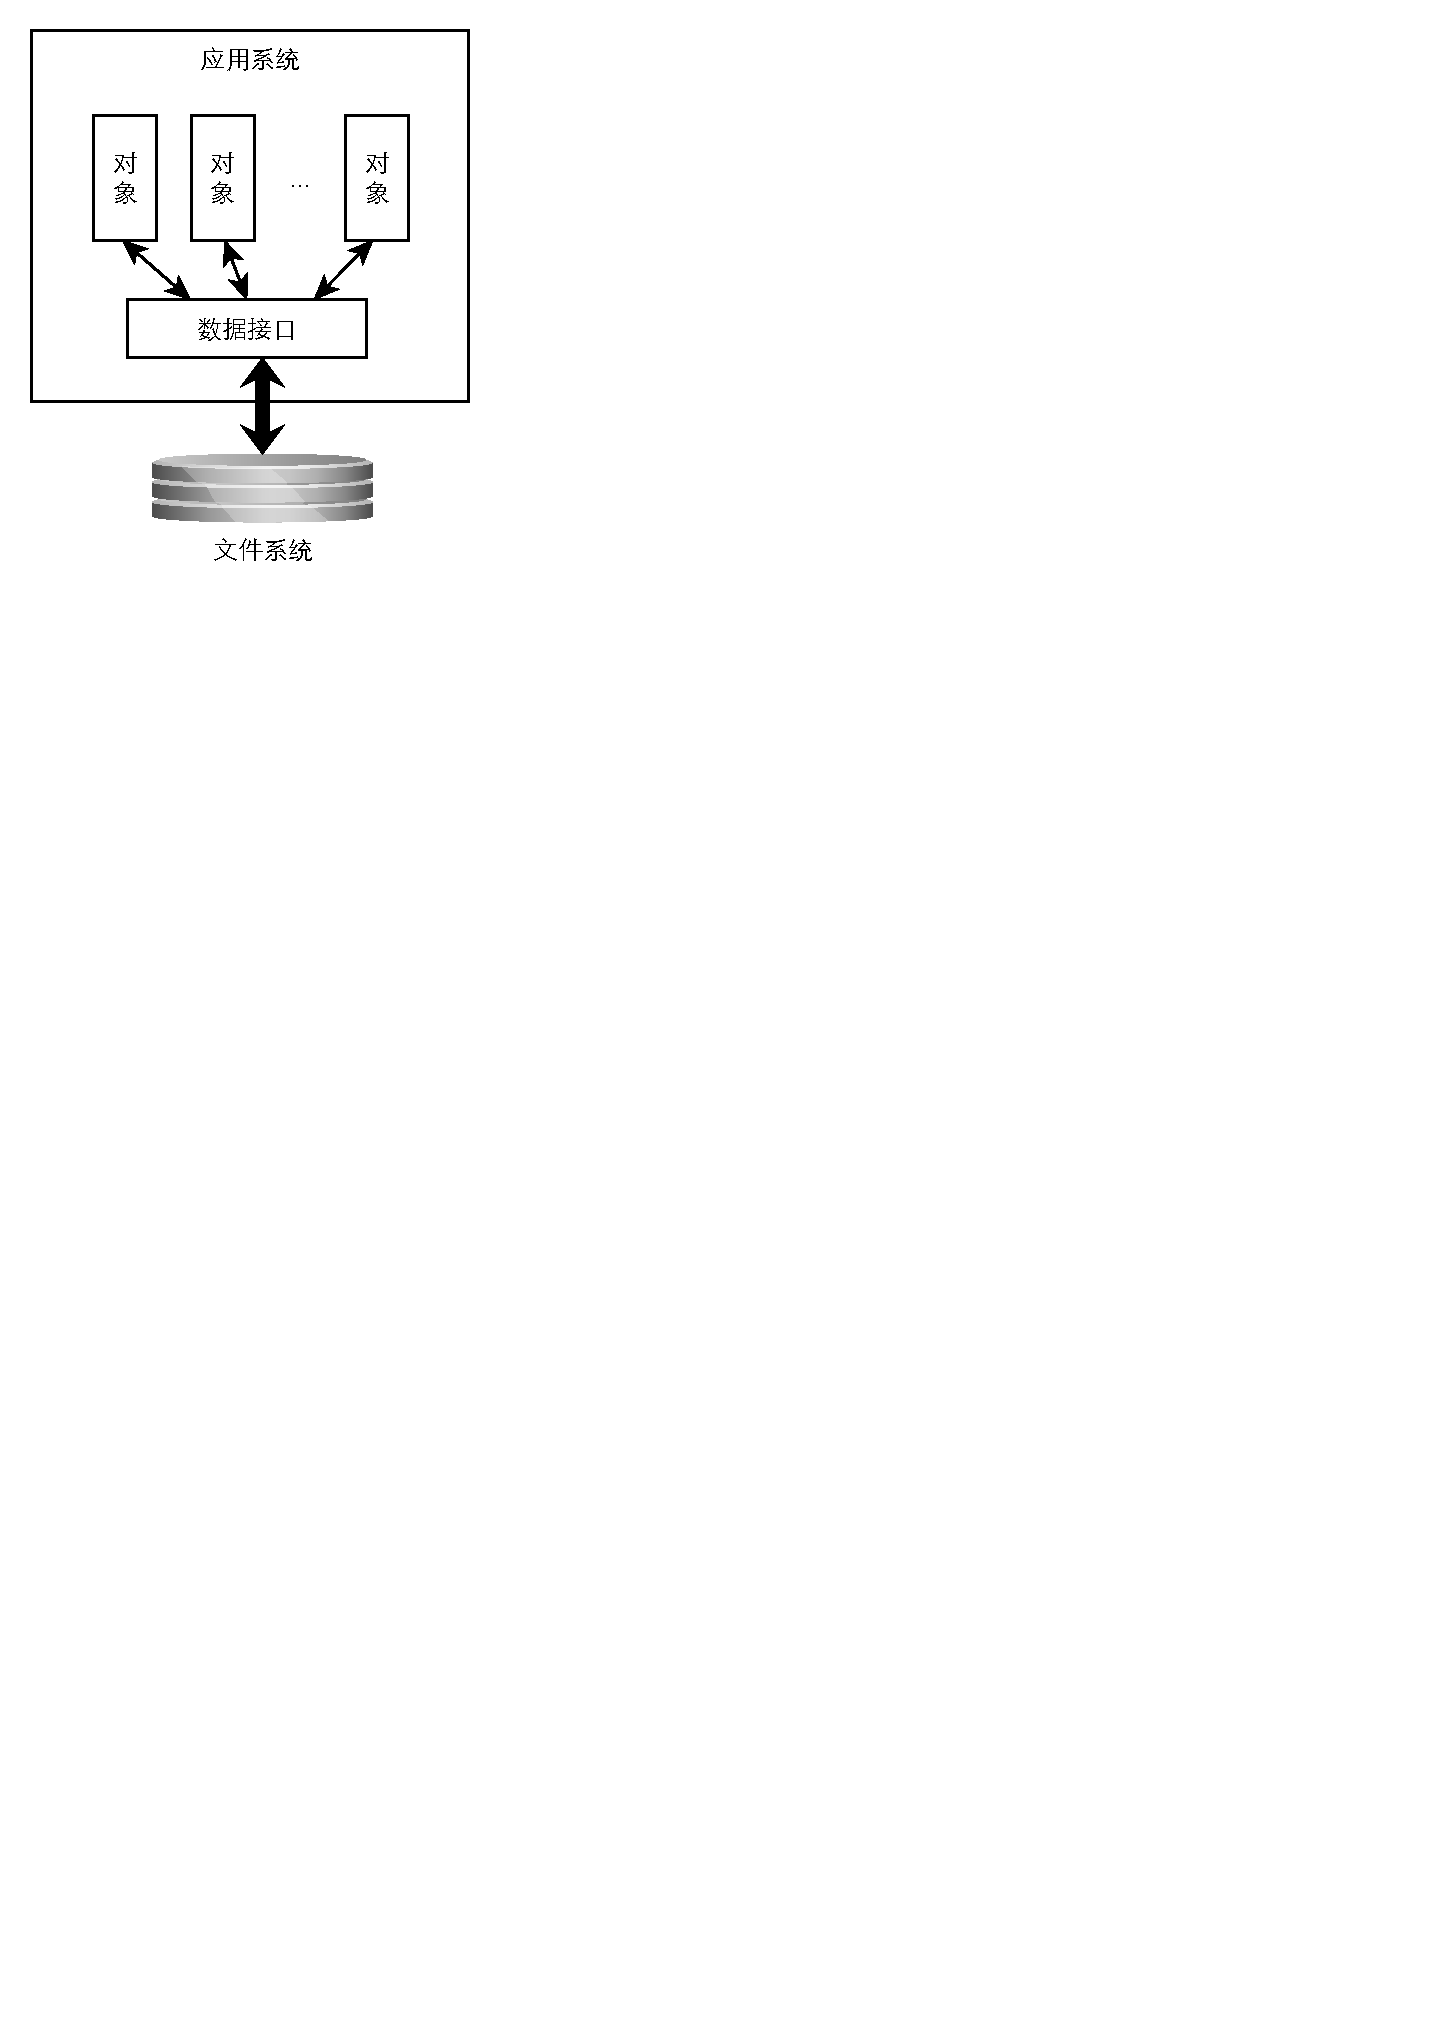
\includegraphics[width=\hsize]{fs.pdf}
\end{columns}
\end{frame}

\begin{frame}
  \frametitle{从应用对象到文件记录的不同映射方式}

  \only<1> {

  \centering\begin{figure}
    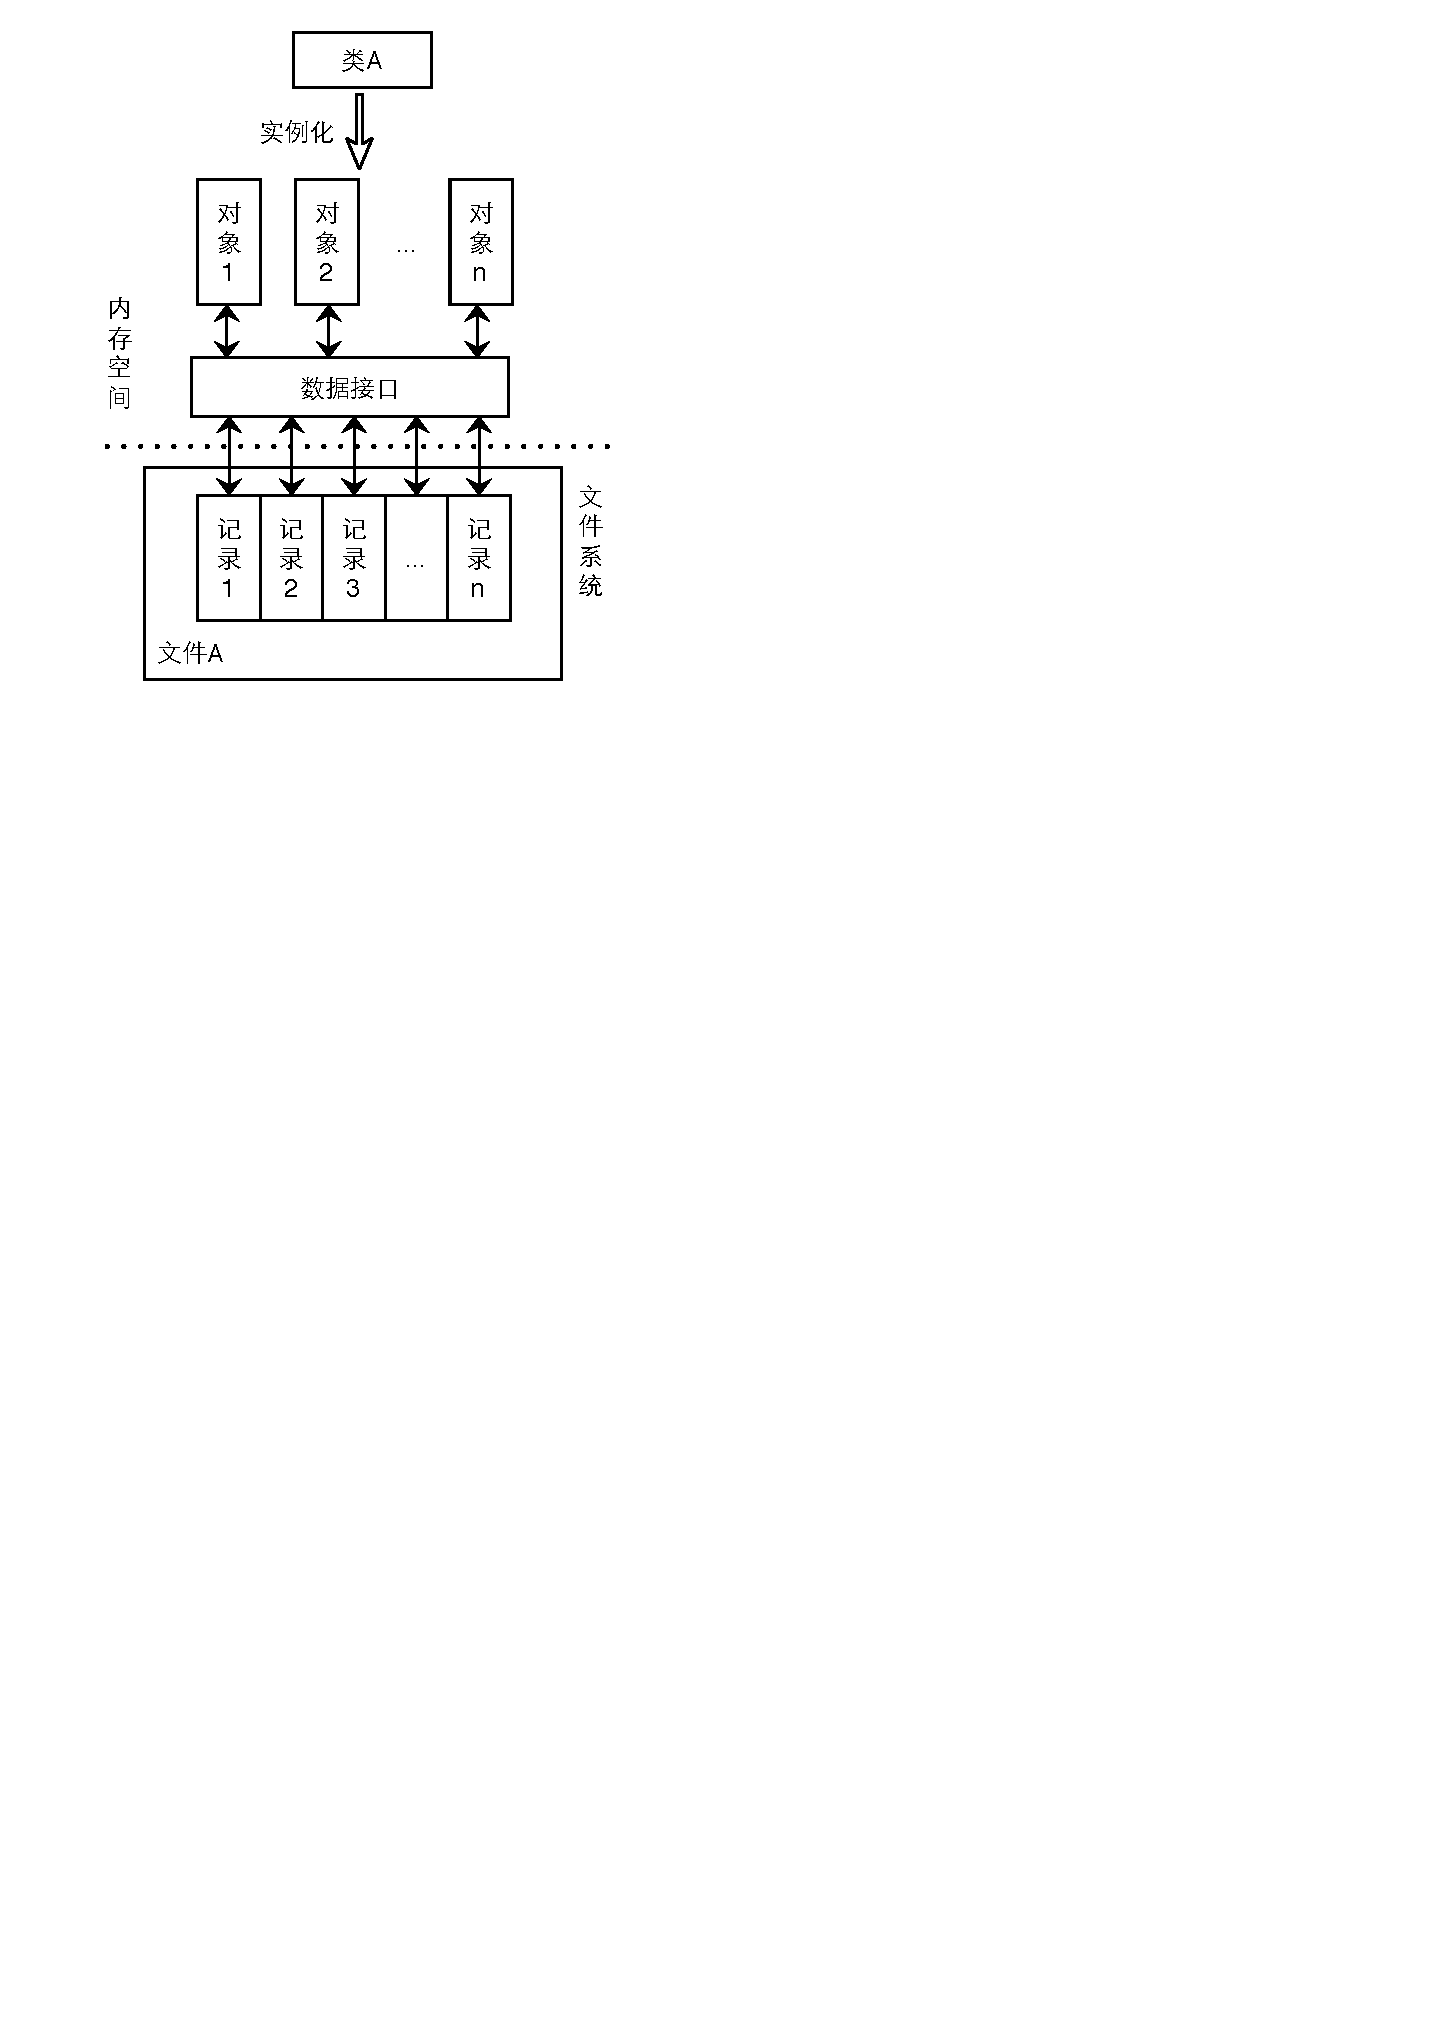
\includegraphics[width=0.4\hsize]{fs-m1.pdf}

    一一对应的映射方式
  \end{figure}
  }

  \only<2> {
    \centering\begin{figure}
    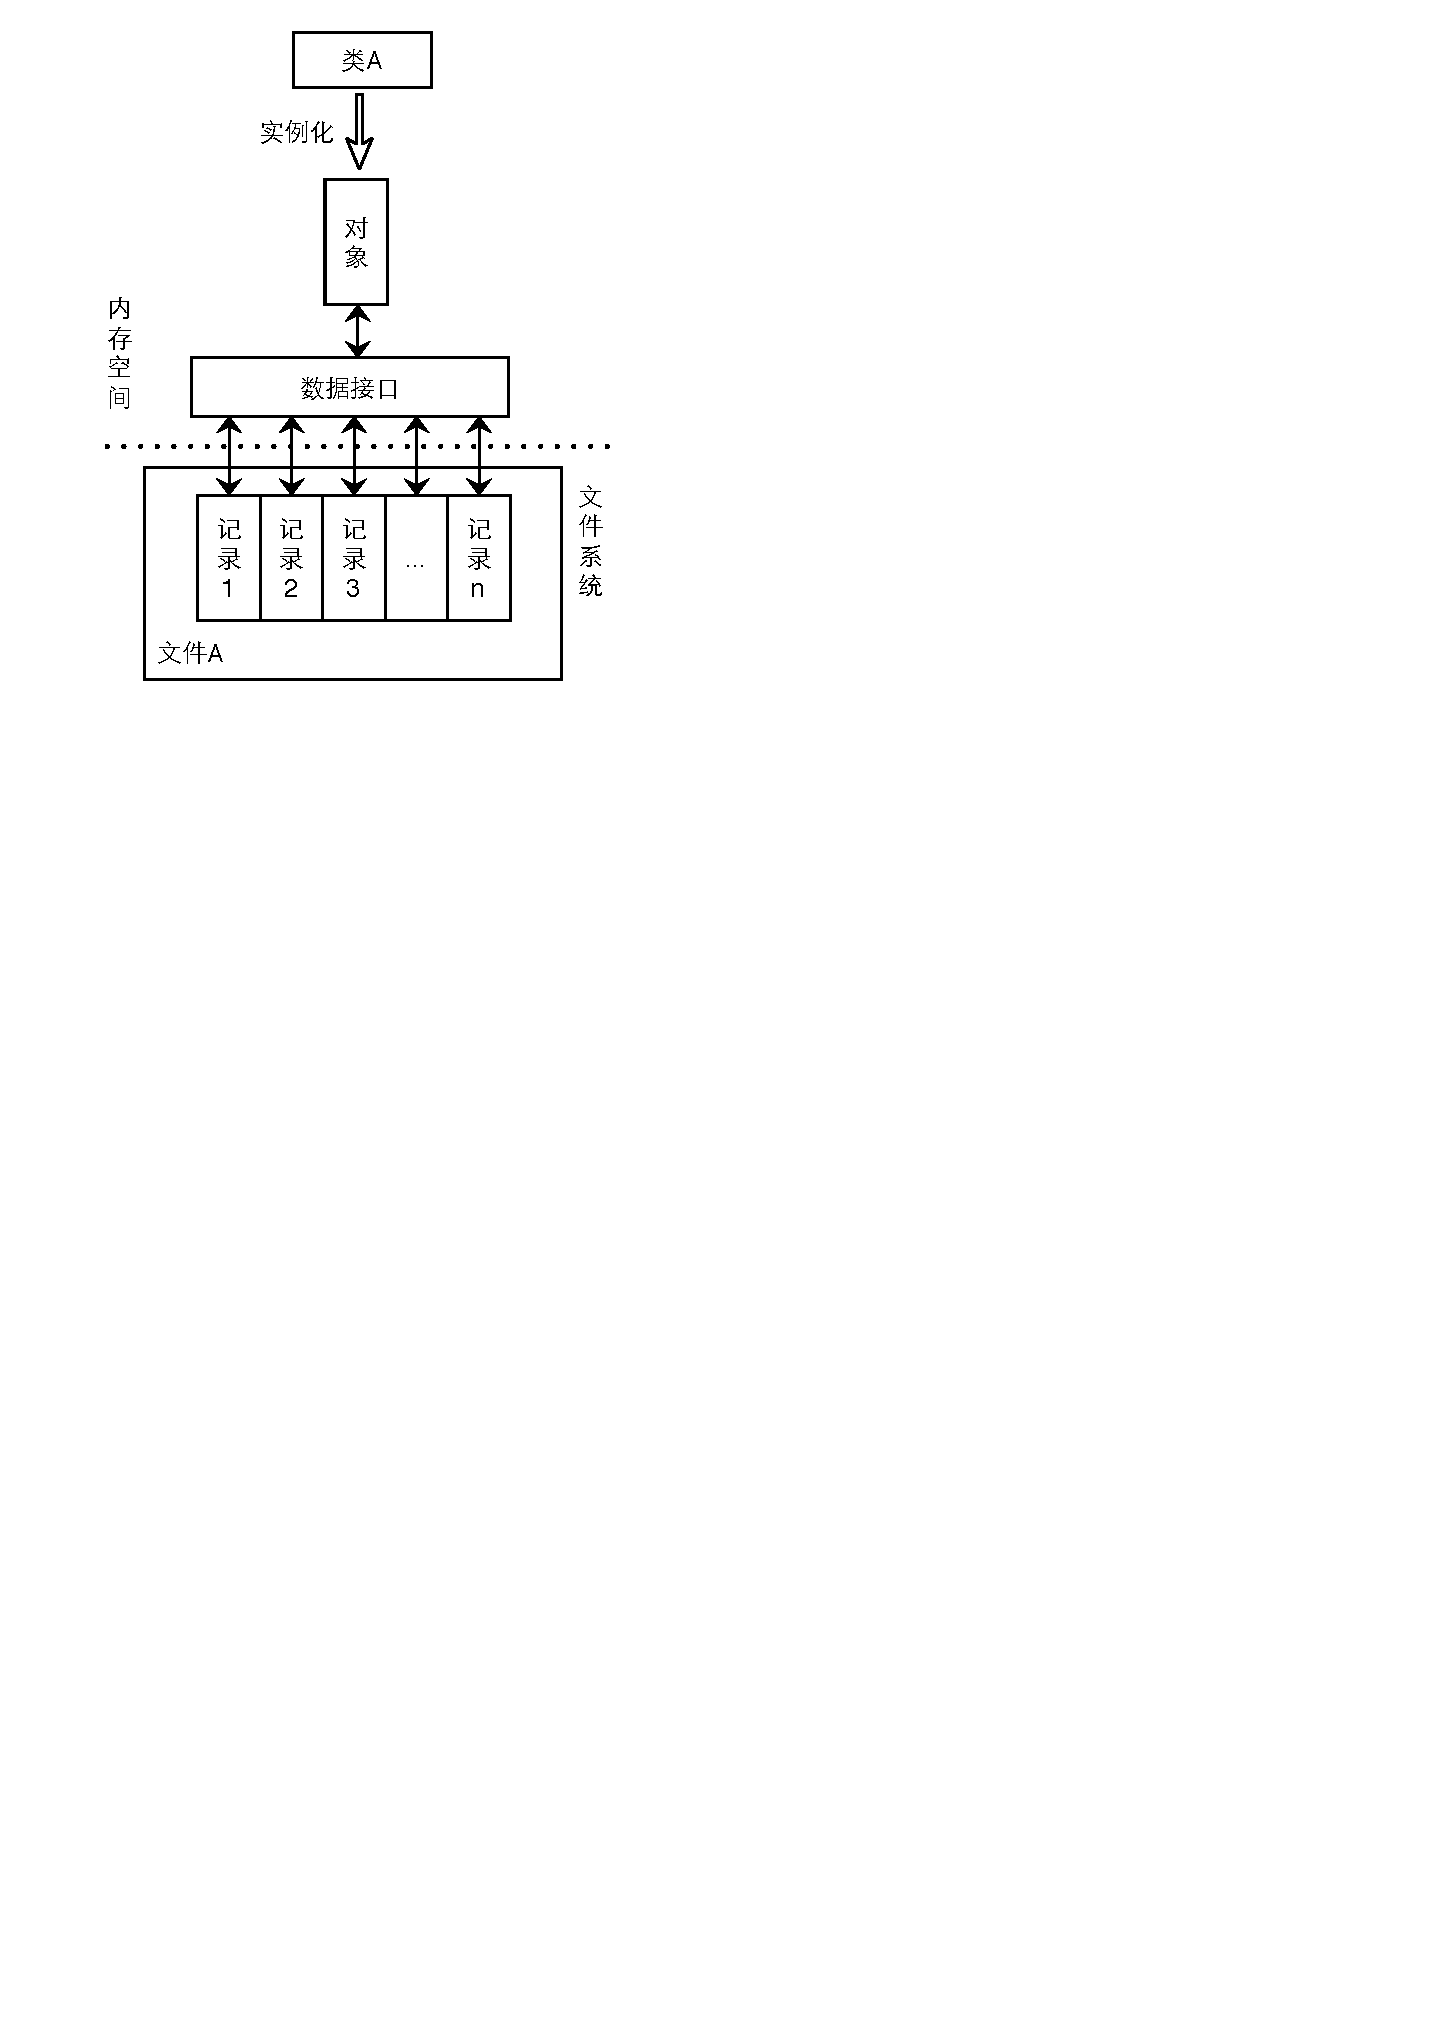
\includegraphics[width=0.4\hsize]{fs-m2.pdf}

    非一一对应的映射方式
  \end{figure}
  }
\end{frame}

\begin{frame}
  \frametitle{对象在文件中的存放策略}

  \only<1> {
    \textbf{基本策略}:  \\[1ex]
  把由每个类直接定义、需要持久存储的全部对象实例存放在一个文件中;
  每个对象实例的全部属性作为一个存储单元,占用该文件的一个记录 \\[2ex]

  \textbf{一般类和特殊类}: \\[1ex]
  每个类各自使用\uline{不同}的文件,分别存放各自直接创建的对象实例
  }

  \only<2> {
    \centering \scalebox{0.8} {
    \begin{tikzpicture}
      \tikzumlset{fill class=white, fill note=white}

      \umlclass[type=abstract]{人员}{姓名}{}

      \umlclass[x=-2, y=-3.5]{研究生}{学号 \\ 班级 \\ 专业}{}
      \umlclass[x=2, y=-3.5]{教职工}{职称 \\ 专业}{}
      \umlclass[y=-7]{在职研究生}{在职单位}{}

      \umlinherit[geometry=|-|]{研究生}{人员}
      \umlinherit[geometry=|-|]{教职工}{人员}
      \umlinherit[geometry=|-|, weight=0.4]{在职研究生}{研究生}
      \umlinherit[geometry=|-|, weight=0.4]{在职研究生}{教职工}

      \umlnote[x=-4, y=-3.5, width=1cm]{研究生}{文件1}
      \umlnote[x=4, y=-3.5, width=1cm]{教职工}{文件2}
      \umlnote[x=3, y=-7, width=1cm]{在职研究生}{文件3}

      \node at (-5,0) {\Large 例:} ;

    \end{tikzpicture}
  }
  }

  \only<3> {
    \textbf{另一种策略}:  \\[1ex]
  一个一般---特殊结构用一个文件,结构中各个类定义的所有对象实例都存放在
  一个文件中\\[2ex]

  \textbf{缺点}: \\[1ex]
  \textcolor{blue}{
  \quad 浪费空间 \\
  \quad 模糊了对象分类关系 \\
  \quad 使操作复杂化 
  }
  }

  \only<4> {
    \textbf{提高检索效率}: 在对象和文件记录间建立有规律的映射关系 
    \begin{itemize}
      \item 对象名或关键字呈线性规律
        \begin{itemize}
          \item 按对象名或关键字的顺序形成文件记录
          \item 给出对象名称或关键字,快速地计算出它的存放位置 
        \end{itemize}
      \item 对象名称或关键字可以比较和排序  
        \begin{itemize}
          \item 按关键字顺序安排记录,检索时采用折半查找法 
          \item 建立按对象名称或者按关键字排序的索引表,通过该表中的记录指针找到相应的记录
        \end{itemize}
      \item 其他措施: 如散列表、倒排表、二叉排序树等等
    \end{itemize}
  }

  
\end{frame}

\begin{frame}
  \frametitle{设计数据接口部分的对象类}
  \noindent\begin{tikzpicture}
    \tikzumlset{fill class=white}

    \umlclass[x=-1]{对象存取器OA}{类名-文件名对照表}{对象存储 \\ 对象恢复}

    \umlclass[y=-4]{查找型OA}{}{对象存储 \\ 对象恢复}
    \umlclass[x=-3, y=-4]{换算型OA}{}{对象存储 \\ 对象恢复}
    \umlclass[x=3, y=-4]{索引型OA}{}{对象存储 \\ 对象恢复}

    \umlclass[x=3]{索引表}{文件记录索引}{查记录指针}
    
    \umlinherit[geometry=|-|]{查找型OA}{对象存取器OA}
    \umlinherit[geometry=|-|, name=inherit]{换算型OA}{对象存取器OA}
    \umlinherit[geometry=|-|]{索引型OA}{对象存取器OA}
    \umluniassoc[anchor1=80, anchor2=-80]{索引型OA}{索引表}

    \umlnote[x=-4.5, width=1.5cm]{对象存取器OA}{负责对象的存储与恢复}
    \umlnote[x=-5.5, y=-3, width=1.5cm]{inherit-2}{子类提供不同查找功能}
  \end{tikzpicture}
\end{frame}

\begin{frame}
  \frametitle{问题域部分的修改}
  \only<1> {
  \scalebox{0.8}{
  \begin{tikzpicture}
    \tikzumlset{fill class=white}
    \umlclass{ClassA}{\textcolor{blue}{ObjectAccess
    oa}}{\textcolor{blue}{ReqSave} \\ \textcolor{blue}{ReqRestore}}
    \umlclass[y=-4]{ClassB}{\textcolor{blue}{ObjectAccess
    oa}}{\textcolor{blue}{ReqSave} \\ \textcolor{blue}{ReqRestore}}

    \umlclass[x=5]{ObjectAccess}{}{}
    \umlsimpleclass[x=4, y=-3, width=1cm]{OA1}
    \umlsimpleclass[x=6, y=-3, width=1cm]{OA2}

    \umlinherit{ClassB}{ClassA}
    \umluniassoc[geometry=-|-]{ClassB}{ObjectAccess}
    \umluniassoc[geometry=-|-]{ClassA}{ObjectAccess}
    \umlinherit[geometry=|-|]{OA1}{ObjectAccess}
    \umlinherit[geometry=|-|]{OA2}{ObjectAccess}

    \draw [dashed] (3, 1) -- (3, -5) ;
    \node [draw, rectangle, rounded corners] at (5, 2) {数据接口部分} ;
    \node [draw, rectangle, rounded corners] at (-4, 2) {问题域部分} ;

    \umlnote[width=3cm, x=-4, y=-2]{ClassA}{策略1: \\每个持久对象类都要增加请求存储和恢复所需
    的属性和操作,以便向数据接口部分发出请求}

  \end{tikzpicture}
  }
}
  \only<2> {
  \scalebox{0.8}{
  \begin{tikzpicture}
    \tikzumlset{fill class=white}
    \umlclass{ClassA}{}{}
    \umlclass[y=-2.5]{ClassB}{}{}

    \umlclass[y=3]{PersistentObject}{\textcolor{blue}{ObjectAccess
    oa}}{\textcolor{blue}{ReqSave} \\ \textcolor{blue}{ReqRestore}}

    \umlclass[x=5]{ObjectAccess}{}{}
    \umlsimpleclass[x=4, y=-2.5, width=1cm]{OA1}
    \umlsimpleclass[x=6, y=-2.5, width=1cm]{OA2}

    \umlinherit{ClassA}{PersistentObject}
    \umlinherit{ClassB}{ClassA}
    \umlinherit[geometry=|-|]{OA1}{ObjectAccess}
    \umlinherit[geometry=|-|]{OA2}{ObjectAccess}
    \umluniassoc[geometry=-|-]{PersistentObject}{ObjectAccess}

    \umlnote[width=2.5cm, x=-4.5]{PersistentObject}{策略2: \\增加一个一般类
    来定义它们,作为共同协议,供所有的持久对象类继承}

    \draw [dashed] (3, 3) -- (3, -3) ;
    \node [draw, rectangle, rounded corners] at (5, 4) {数据接口部分} ;
    \node [draw, rectangle, rounded corners] at (-4.5, 4) {问题域部分} ;
  \end{tikzpicture}
  }
}
\end{frame}

\subsection[RDBMS]{针对RDBMS的设计}

\begin{frame}
  \frametitle{如何看待用RDBMS存储对象}
  \begin{columns}[t]
    \column{0.6\hsize}

  对象在内存空间和数据库的映像
  \begin{itemize}
    \item 应用系统仍然是面向对象的
    \item 只是用关系数据库存储对象的数据
  \end{itemize}

    \column{0.4\hsize}

  \centering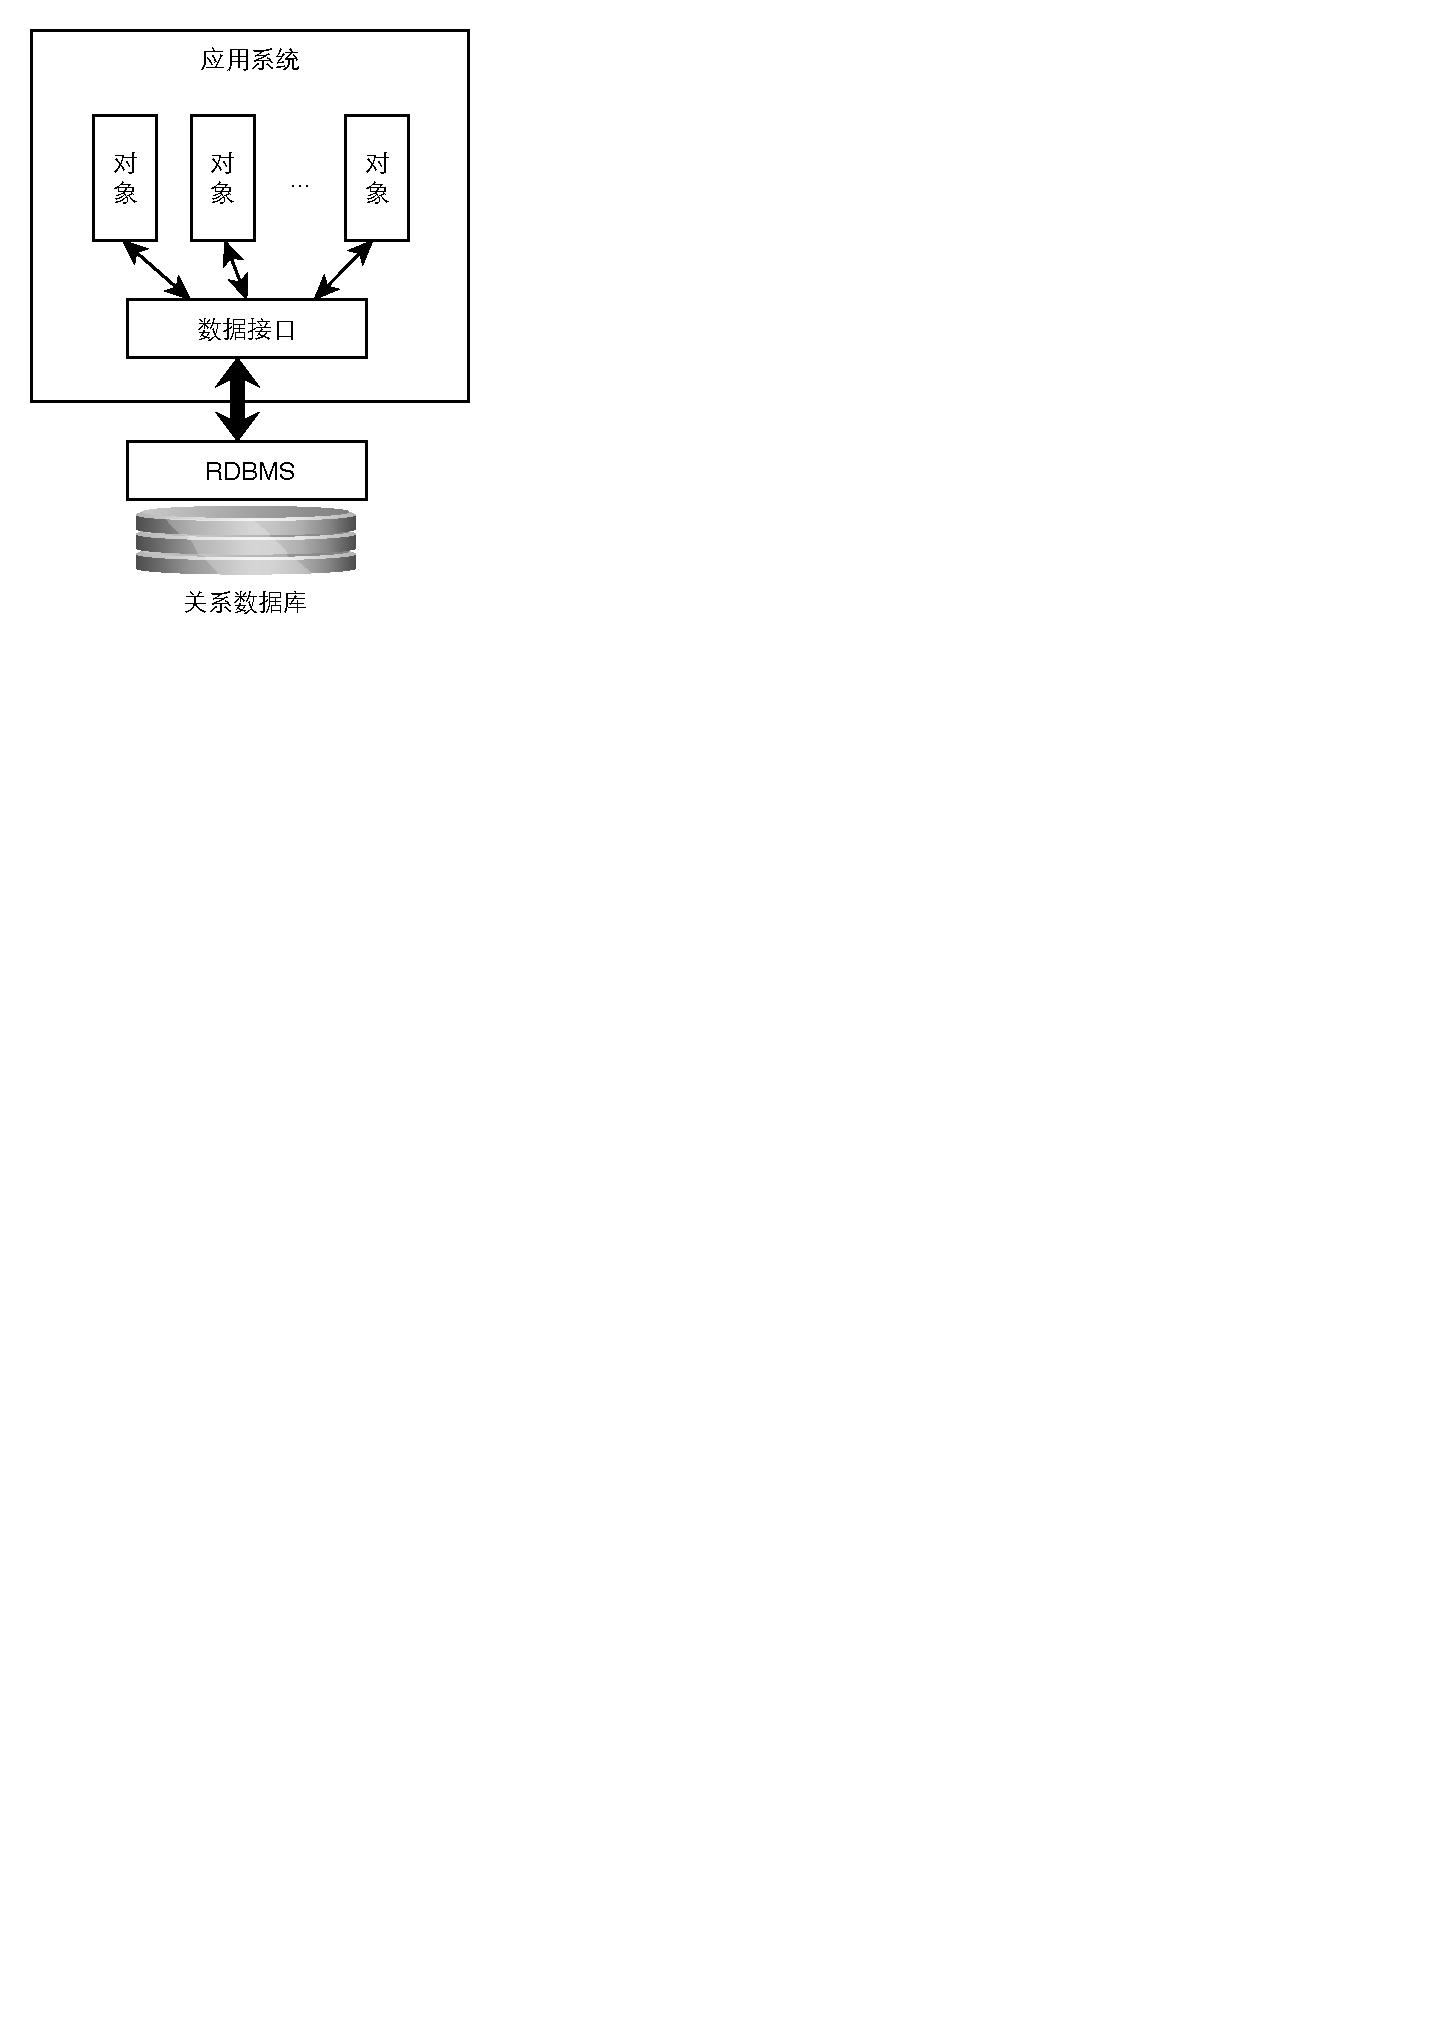
\includegraphics[width=\hsize]{rdbms.pdf}
\end{columns}
\end{frame}

\begin{frame}
  \frametitle{从应用对象到数据库表元组的不同映射方式}

  \only<1> {

  \centering\begin{figure}
    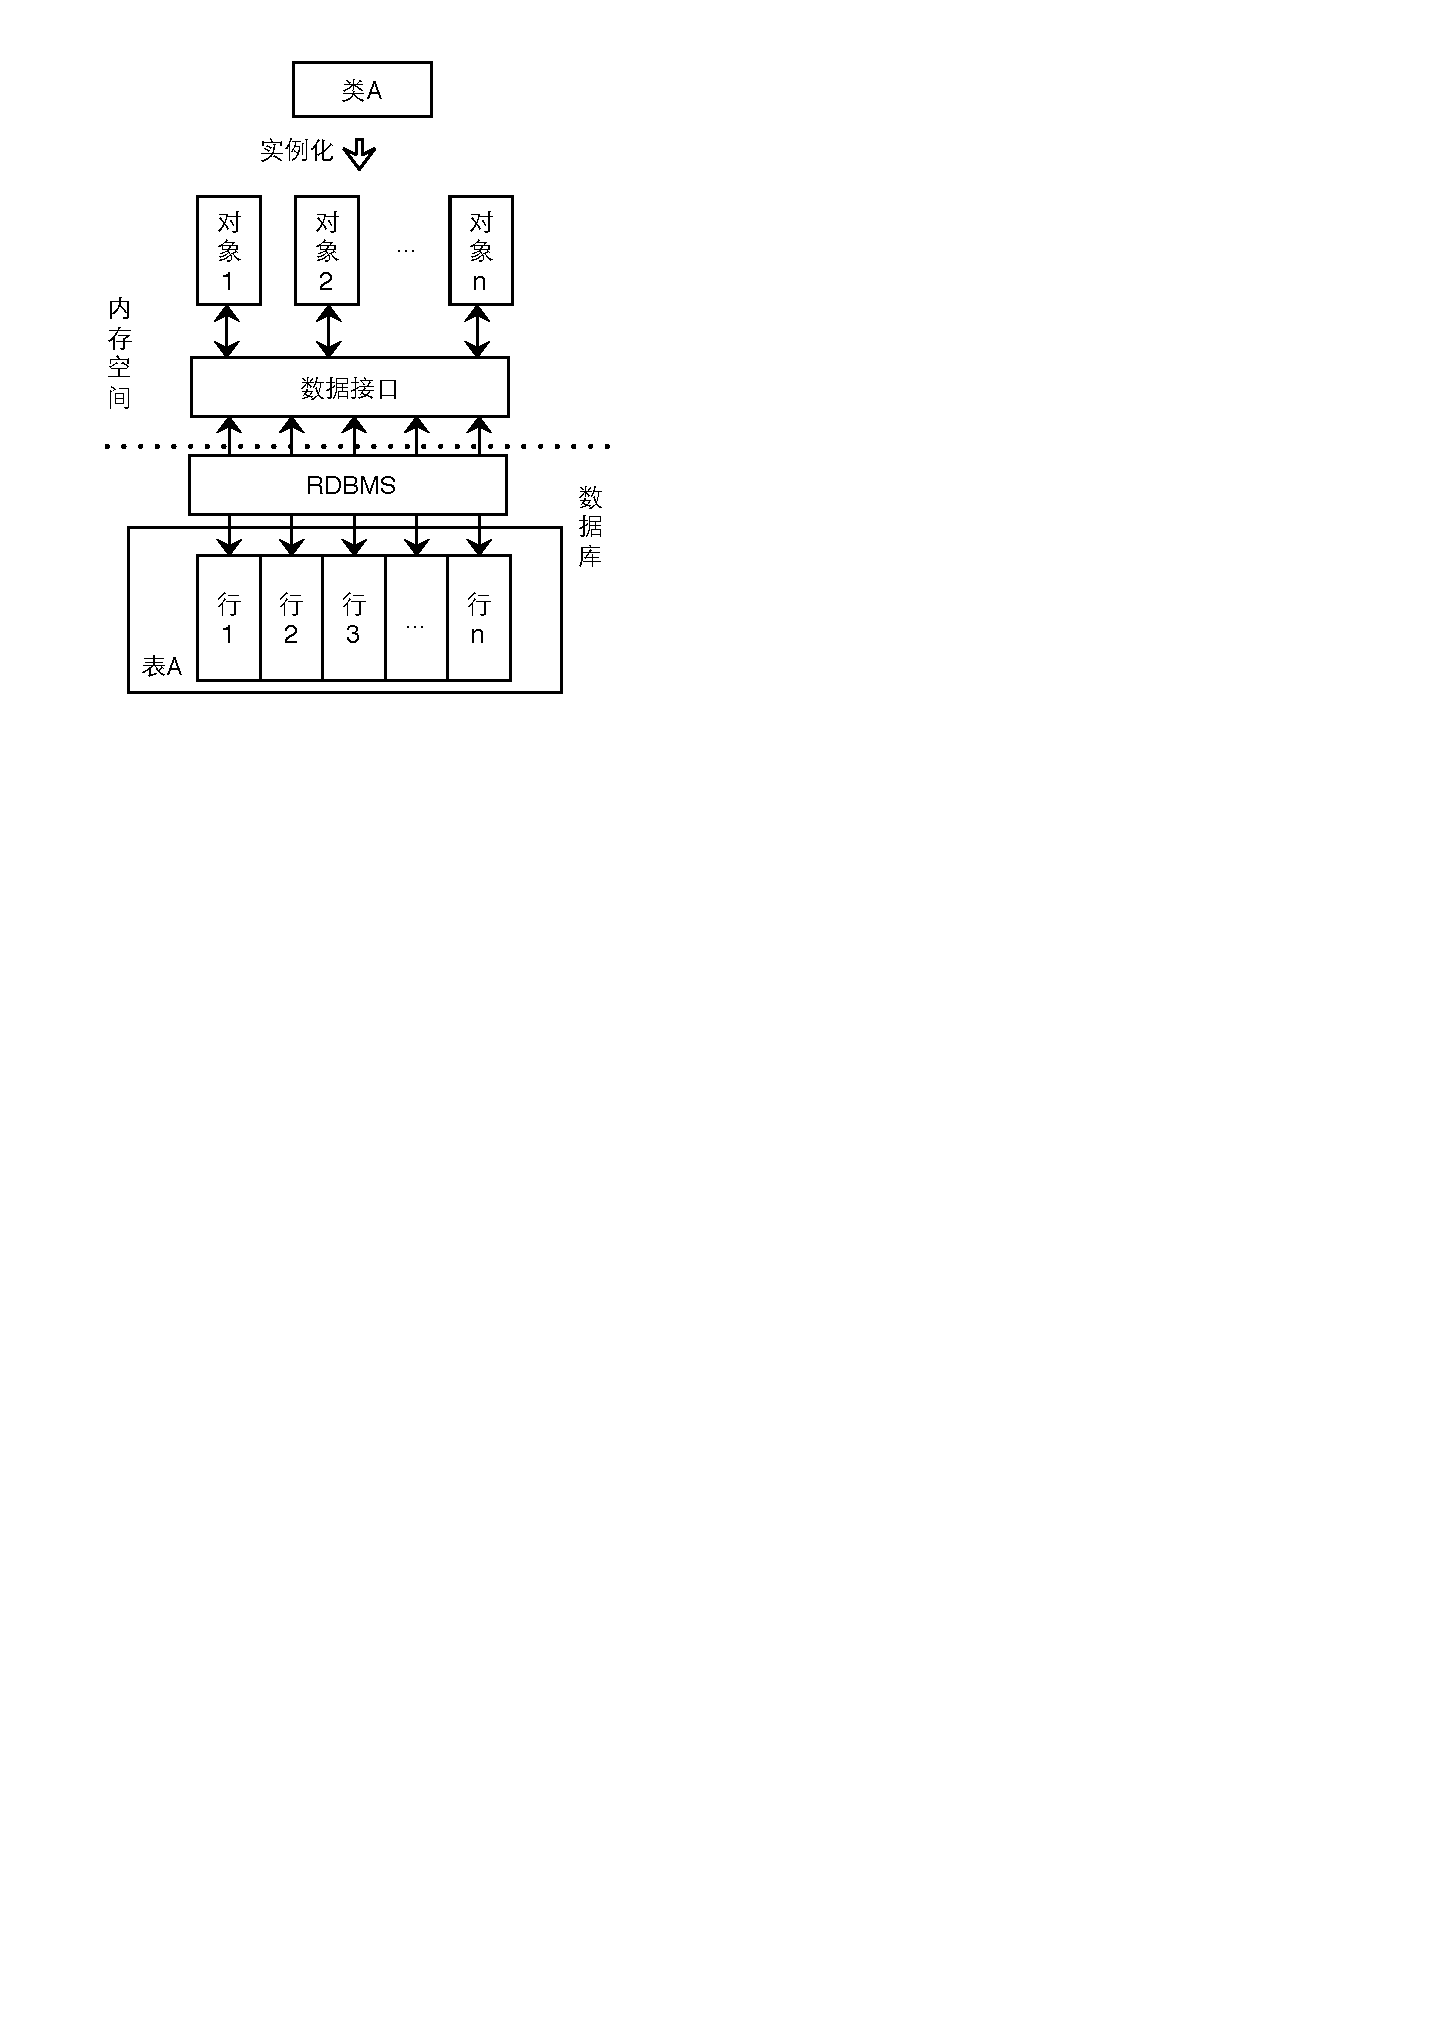
\includegraphics[width=0.45\hsize]{rdbms-m1.pdf}

    一一对应的映射方式
  \end{figure}
  }

  \only<2> {
    \centering\begin{figure}
    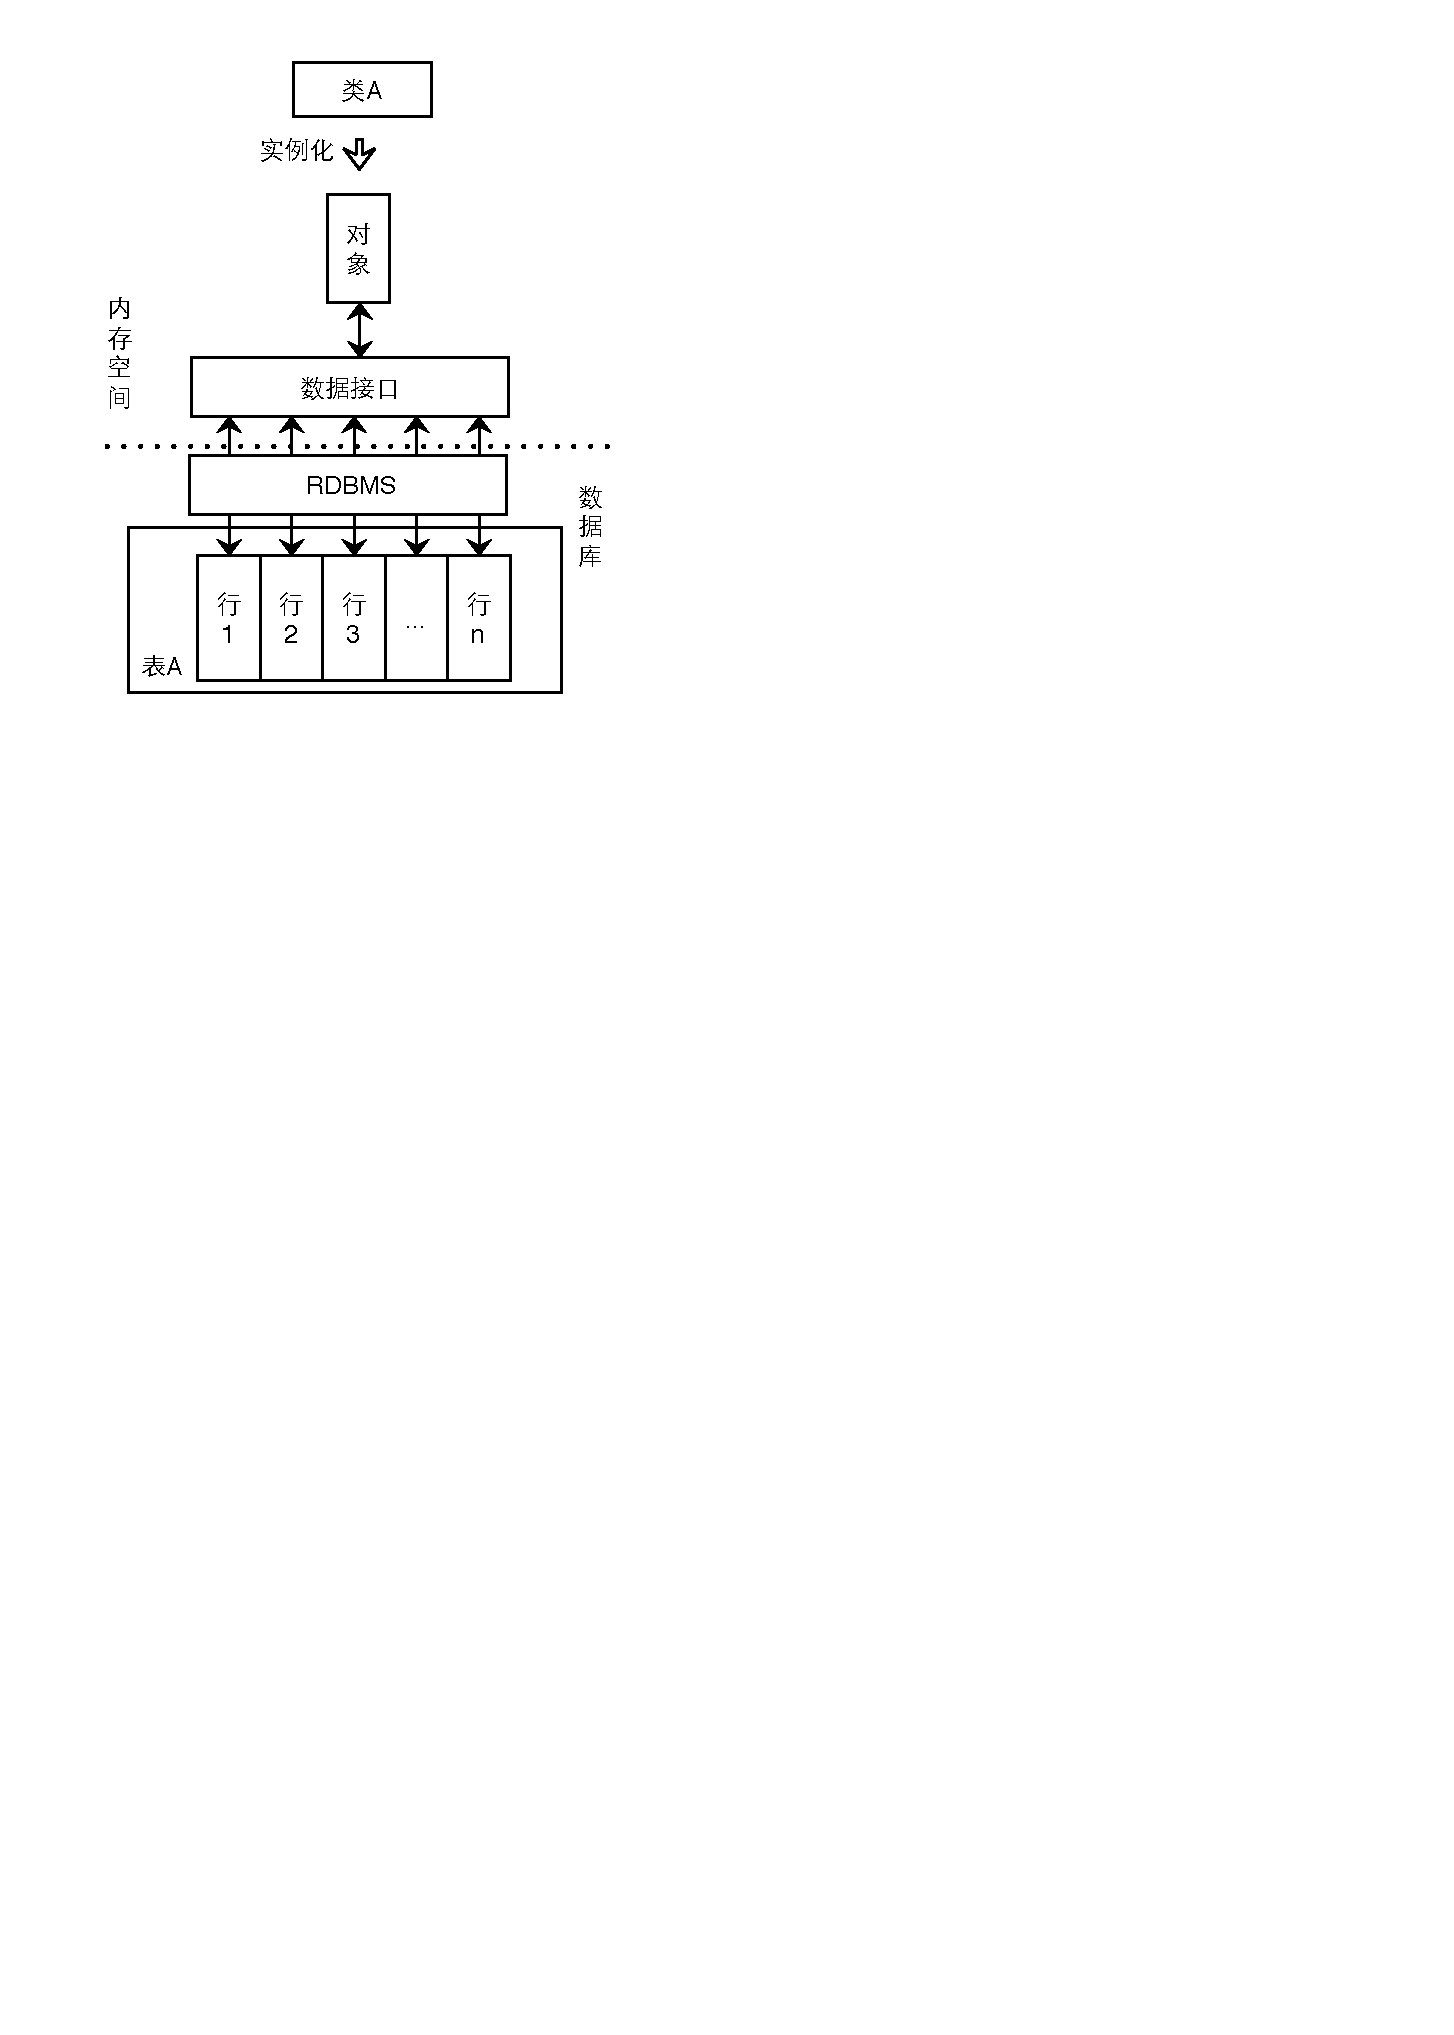
\includegraphics[width=0.45\hsize]{rdbms-m2.pdf}

    非一一对应的映射方式
  \end{figure}
  }
\end{frame}

\begin{frame}
  \frametitle{使用RDBMS与文件系统的比较}

  \begin{enumerate}
    \item 系统以不同方式使用数据库中的数据
      \begin{itemize}
        \item 把数据库中已有的数据描述为本系统中的类和对象
        \item 系统中的对象直接使用数据库中的普通数据,二者之间不存在直接
          映射关系,只是一种简单的\uline{使用关系}
      \end{itemize}
    \item 为了满足关系数据库对\uline{规范化}的要求,可能需要数据格式的转换
      \begin{itemize}
        \item 只限于一个类的范围的情况
        \item 牵涉到多个类的情况
      \end{itemize}
  \end{enumerate}
\end{frame}

\begin{frame}
  \frametitle{对象在数据库中的存放策略}
  \begin{itemize}
    \item 对象数据的规范化
    \item 修改类图
    \item 确定关键字
    \item 从类图映射到数据库表
      \begin{itemize}
        \item 类 $\rightarrow$ 表
        \item 类的属性 $\rightarrow$ 表的属性
        \item 对象实例 $\rightarrow$ 行
        \item 对一般-特殊结构、整体-部分结构、关联等OO概念的处理
      \end{itemize}
  \end{itemize}
\end{frame}

\begin{frame}
  \frametitle{对象数据的规范化}
  \only<1> {
    关系数据库要求存入其中的数据符合一定的规范,并且用\textcolor{blue}{范式}衡量规范化程度
    的高低 \\[2ex]
    \textcolor{blue}{第一范式}(1NF): 属性是\uline{原子}的,不可再分 \\[2ex]

    不符合第一范式的例子:\\[3ex]

    \begin{tabular}{|c|c|}
      \hline
    姓名 & 电话 \\ \hline \hline
    张三 & \hspace*{2ex} 18900010002 \hspace*{2ex} \vline \hspace*{2ex} 62750114
    \hspace*{2ex} \\ \hline
  \end{tabular}

}
 
\only<2-3> {
  \textcolor{blue}{第二范式}(2NF):非关键属性\uline{完全依赖}整个关键字,
  即不能依赖关键属性的一部分,意味着一个表只描述一个事物 \\[2ex]

    不符合第二范式的例子:\\[2ex]

    \begin{tabular}{|c|c|c|c|c|c|}
      \hline
      学号 & 姓名 & 年龄 & 课程 & 成绩 & 学分 \\ \hline \hline
     1010 & 张三 & 19 & 英语 & 88 & 4 \\
    \hline
  \end{tabular}
}

\only<3> {
  \vspace*{2ex}
  修正: \\[2ex]
    \begin{tabular}{|c|c|c|}
      \hline
      学号 & 姓名 & 年龄 \\ \hline \hline
     1010 & 张三 & 19  \\
    \hline
  \end{tabular}
    \begin{tabular}{|c|c|}
      \hline
      课程 & 学分 \\ \hline \hline
     英语 & 4  \\
    \hline
  \end{tabular}
    \begin{tabular}{|c|c|c|}
      \hline
      学号 & 课程 & 成绩 \\ \hline \hline
     1010 & 英语 & 88  \\
    \hline
  \end{tabular}
}

  \only<4-5> {
    \textcolor{blue}{第三范式}(3NF):不存在非关键属性对任一
    候选关键属性的\uline{传递依赖},即属性不依赖于其它非关键属性 \\[2ex]

    不符合第三范式的例子:\\[2ex]

    \begin{tabular}{|c|c|c|c|c|c|}
      \hline
      学号 & 姓名 & 年龄 & 所在学院 & 学院地点 & 学院电话 \\ \hline \hline
     1010 & 张三 & 19 & 信科 & 理科2号楼 & 62751760 \\
    \hline
  \end{tabular}

}

\only<5> {
  \vspace*{2ex}
  修正: \\[2ex]
  \small
    \begin{tabular}{|c|c|c|c|}
      \hline
      学号 & 姓名 & 年龄 & 学院 \\ \hline \hline
     1010 & 张三 & 19  & 信科 \\
    \hline
  \end{tabular}
  \begin{tabular}{|c|c|c|}
      \hline
      学院 & 地点 & 电话\\ \hline \hline
     信科 & 理科2号楼 & 62751760  \\
    \hline
  \end{tabular}
}


  \only<6> {
    \textcolor{blue}{Boyce-Codd范式}(BCNF):
    \uline{所有属性}(包括关键属性)都不传递依赖于任何候选关键字 \\[2ex]

    不满足BCNF范式的例子: \\
    某仓库管理系统,一个管理员只在一个仓库工
    作;一个仓库可以存储多种物品\\[2ex]

    \begin{tabular}{|c|c|c|c|}
      \hline
      仓库ID & 管理员ID & 存储物品ID & 数量 \\ \hline \hline
     10 & 张三 & BMWX5 & 10 \\
    \hline
  \end{tabular}


  }

  \only<7-8> {
    \textcolor{blue}{第四范式}:是第三范式,且表中不能包含一个实体的多个
    互相独立的值 \\[2ex]

    不满足第四范式的例子及其规范化:\\[2ex]

    \small

    \begin{tabular}{|c|c|c|}
      \hline
      学号 & 课程 & 活动 \\ \hline \hline
     100 & 音乐 & 游泳 \\ \hline
     100 & 会计 & 游泳 \\ \hline
     100 & 音乐 & 网球 \\ \hline
     100 & 会计 & 网球 \\ \hline
     100 & 音乐 & 桥牌 \\ \hline
     100 & 会计 & 桥牌 \\ \hline
  \end{tabular}%
}
  \only<8> {
  {\hspace*{2ex}$\Rightarrow$\hspace*{2ex}}
    \begin{tabular}{|c|c|}
      \hline
      学号 & 课程 \\ \hline \hline
     100 & 音乐 \\ \hline
     100 & 会计 \\ \hline
  \end{tabular}%
  \hspace*{2ex}  \begin{tabular}{|c|c|}
      \hline
      学号 & 活动 \\ \hline \hline
     100 & 游泳 \\ \hline
     100 & 网球 \\ \hline
     100 & 桥牌 \\ \hline
  \end{tabular}%
  }

  \only<9> {
    用面向对象方法得到的分类 \\[2ex]
    \begin{tikzpicture}
      \tikzumlset{fill class=white}

      \umlemptyclass{学生}
      \umlemptyclass[x=-3]{课程}
      \umlemptyclass[x=3]{活动}

      \umlassoc[mult1=*, mult2=*]{学生}{课程}
      \umlassoc[mult1=*, mult2=*]{学生}{活动}
    \end{tikzpicture}

    化解多对多关联后 \\[2ex]
  \noindent\begin{tikzpicture}
      \tikzumlset{fill class=white}

      \umlemptyclass[width=1cm]{学生}
      \umlemptyclass[x=-2.5]{学生课程}
      \umlemptyclass[x=2.5]{学生活动}
      \umlemptyclass[x=5, width=1cm]{活动}
      \umlemptyclass[x=-5, width=1cm]{课程}

      \umlassoc[mult1=1, mult2=*]{学生}{学生课程}
      \umlassoc[mult1=1, mult2=*]{学生}{学生活动}
      \umlassoc[mult1=1, mult2=*]{活动}{学生活动}
      \umlassoc[mult1=1, mult2=*]{课程}{学生课程}
    \end{tikzpicture}
  }

  \only<10> {
    面向对象虽然可以得到符合较高范式要求的数据库表,但面向对象方法并不总
    是能得到规范化的结果 \\[4ex]

    \centering\begin{tikzpicture}
      \umlclass[fill=white]{职工}{职工编号 \\
        月工资\\
      所得税}{}
    \end{tikzpicture}
  }

  \only<11> {

    小结 

    \begin{itemize}
      \item 未必规范化程度越高越好
        \begin{itemize}
          \item 规范化可能影响系统的可理解性,另外增加了多表查询和连接操作
        \end{itemize}

      \item 面向对象方法与关系数据库的规范化目标既有相违的一面,又有相符的一面 
        \begin{itemize}
          \item 对象的数据结构常常连1NF的要求都不能满足 
          \item 以对象为中心组织数据与操作,可能有助于达到第2、3等范式的
            要求
        \end{itemize}
    \end{itemize}
}

\end{frame}

\begin{frame}
  \frametitle{修改类图}
  \only<1> {
  规范化可能引发对类图的修改

  \begin{enumerate}
    \item 保持类图,对表规范化 \\
   缺点是对象的存储与恢复必须经过数据格式的转换 

    \item 修改类图 \\
   对问题域的映射可能不像规范化之前那么直接。但是这个问题并不严重
  -- 利大于弊
    \item 确定关键字 \\
      用较少的属性作为关键字将为含关键字的操作带来方便
  \end{enumerate}
}

  \only<2> {
    \textbf{最终效果:} \\
    经过必要的规范化处理和关键字处理之后,得到一个符合数据库设计要求的类
    图,其中每个需要映射到数据库表的类,都满足如下条件:
    \begin{itemize}
      \item 至少满足第一范式
      \item 满足所期望的更高范式
      \item 有一组属性被确定为关键字
    \end{itemize}
  }

\end{frame}

\begin{frame}
  \frametitle{从类图到数据库的映射策略}
  \begin{itemize}
    \item 对每个要在数据库中存储对象实例的类,都建立一个数据库表

    \item 类的每个属性(包括从所有祖先继承来的属性)都对应表的一个属性(列)
      \begin{itemize}
        \item 名称、数据类型完全相同
        \item 其中一组属性被确定为关键字
      \end{itemize}

    \item 类的每个对象实例将对应表的一个元组(行)
  \end{itemize}
\end{frame}

\begin{frame}
  \frametitle{从类图到数据库映射中类图的处理}
  主要考虑:
  \begin{itemize}
    \item 一般--特殊结构
    \item 关联
    \item 整体--部分结构
  \end{itemize}
\end{frame}

\begin{frame}
  \frametitle{对一般--特殊结构的处理}
  \framebox{\parbox{0.8\hsize}{\centering 抽象类\alert{\sout{不对应}}数据库表 \\
    特殊类包括自己定义的和继承来的\textcolor{blue}{所有}属性}}

    \vspace*{2ex}

    \noindent\begin{tikzpicture}
      \tikzumlset{fill class=white}

      \umlclass[type=abstract]{人员}{姓名\\出生日期}{}
      \umlclass[x=-4.5, y=-1]{研究生}{学号\\班级\\攻读专业}{}
      \umlclass[x=4.5, y=-1]{教职工}{职称\\保险记录\\从事专业}{}
      \umlclass[y=-3]{在职研究生}{在职单位}{}

      \umlinherit{研究生}{人员}
      \umlinherit{教职工}{人员}
      \umlinherit{在职研究生}{研究生}
      \umlinherit{在职研究生}{教职工}

      \umlnote[x=-2.4, y=0.5, width=1.2cm]{人员}{不建表}
      \umlnote[x=4.5, y=-3.5, width=1.5cm]{教职工}{5个属性}
      \umlnote[x=-4.5, y=-3.5, width=1.5cm]{在职研究生}{9个属性}
    \end{tikzpicture}
\end{frame}

\begin{frame}
  \frametitle{对关联的处理}

  \begin{enumerate}
    \item 在关联连接线一端的类中定义一个(或一组)属性,表明另一端类的哪个对象实
  例与本端的对象实例相关联
  \begin{itemize}
    \item 该属性(属性组)应该和另一端的关键字相同
    \item 如果另一端的关键字包含多个属性,本端也要定义同样的多个属性
  \end{itemize}
    \item 在对应的数据库表中,一个表以该属性(或属性组)作为
      \textbf{\textcolor{blue}{外键}
      },另一个表以它作
      为\textbf{\textcolor{blue}{主键}},使前者的元组通过其属性值指向后者的元组 
\end{enumerate}

\end{frame}

\begin{frame}
  \frametitle{一对一的关联}
  \centering\begin{tikzpicture}
    \tikzumlset{fill class=white}
    \umlemptyclass{A}
    \umlemptyclass[x=4]{B}
    \umluniassoc[mult1=0..1, mult2=1]{A}{B}
  \end{tikzpicture}

  \vspace*{4ex}

  \centering\begin{tikzpicture} [scale=0.5]
  \draw (-2,-2) grid (3,2) ;
  \draw (8,-2) grid (12,2) ;

  \filldraw [red] (1.5,0.5) circle [radius=3pt] ;

  \draw[->, thick, >=Stealth] (1.5,0.5) .. controls (5, 0.5) and
  (4,-0.5) .. (8, -0.5);

  \node at (0.5,-3) {表A} ;
  \node at (10,-3) {表B} ;
  \end{tikzpicture}
\end{frame}

\begin{frame}
  \frametitle{一对多的关联}
  从多重性约束为 \textcolor{blue}{$m$} 的一端指向多重性约束为
  \textcolor{blue}{1} 的一端 \\[2ex]

  \centering\begin{tikzpicture}
    \tikzumlset{fill class=white}
    \umlemptyclass{A}
    \umlemptyclass[x=4]{B}
    \umluniassoc[mult1=*, mult2=1]{A}{B}
  \end{tikzpicture}

  \vspace*{2ex}

  \centering\begin{tikzpicture} [scale=0.5]
  \draw (-2,-2) grid (3,2) ;
  \draw (8,-2) grid (12,2) ;

  \filldraw [red] (1.5,0.5) circle [radius=3pt] ;

  \draw[->, thick, >=Stealth] (1.5,0.5) .. controls (5, 0.5) and
  (4,-0.5) .. (8, -0.5);

  \node at (0.5,-3) {表A} ;
  \node at (10,-3) {表B} ;
  \end{tikzpicture}

  映射为数据库表后,
  A表以B表的主键作为自己的外键

\end{frame}

\begin{frame}
  \frametitle{多对多的关联}

  \only<1> {
  先将多对多关联化为两个1对多的关联 \\[2ex]

  \centering\begin{tikzpicture}
    \tikzumlset{fill class=white}
    \umlemptyclass{A}
    \umlemptyclass[x=4]{B}

    \umlassoc[mult1=*, mult2=*]{A}{B}
  \end{tikzpicture}

  \alert{$\Downarrow$} \\[3ex]

  \centering\begin{tikzpicture}
    \tikzumlset{fill class=white}
    \umlemptyclass{AB}
    \umlemptyclass[x=3]{B}
    \umlemptyclass[x=-3]{A}

    \umluniassoc[mult1=*, mult2=1]{AB}{B}
    \umluniassoc[mult1=*, mult2=1]{AB}{A}
  \end{tikzpicture}
  }

  \only<2> {
    然后将每个类映射到一个数据库表 \\[3ex]

  \centering\begin{tikzpicture} [scale=0.5]
  \draw (-1,-2) grid (1,2) ;
  \draw (7,-1) grid (10,1) ;
  \draw (-7,-1) grid (-10,1) ;

  \filldraw [red] (0.5,0.5) circle [radius=3pt] ;
  \filldraw [red] (-0.5,0.5) circle [radius=3pt] ;

  \draw[->, thick, >=Stealth] (0.5,0.5) .. controls (5, 0.5) and
  (4,-0.5) .. (7, -0.5);
  \draw[->, thick, >=Stealth] (-0.5,0.5) .. controls (-5, 0.5) and
  (-4,-0.5) .. (-7, -0.5);

  \node at (0,-3) {表AB} ;
  \node at (8.5,-3) {表B} ;
  \node at (-8.5,-3) {表A} ;
  \end{tikzpicture}
  
  \vspace*{3ex}

  AB表含有两个外键,一个是A的主键,一个是B的主键
  }

  \only<3> {
    对象类转化为数据库表的几种情况:
    \begin{itemize}
      \item 表中只包含描述本类事物自身特征的属性
      \item 表中既包含描述本类事物自身特征的属性,
       也包含作为外键指向另一个表的元组的属性
     \item 表中只包含作为外键指向其它表的元组的属性
   \end{itemize}
  }
\end{frame}

\begin{frame}
  \frametitle{对整体-部分结构的处理}

  \only<1> {
  分为 \textcolor{blue}{紧密、固定}的方式 和 \textcolor{blue}{松散、灵活
  }的方式

  \begin{block}{紧密、固定方式}
    把部分对象类的属性\textcolor{blue}{合并}到整体对象类中
  \end{block}

  \begin{block}{松散、灵活方式}
  整体对象类和部分对象类分别建立一个表,
  通过\textcolor{blue}{外键}表现整体-部分关系
  \end{block}

  多重性约束对实现方式也有影响,紧密、固定的实现方式适合1对1的组合关系
  }

  \only<2> {
    \begin{tikzpicture}
      \tikzumlset{fill class=white, fill note=white}

      \umlemptyclass{A}
      \umlemptyclass[x=3]{B}

      \umlcompo[mult1=1, mult2=1, name=compo]{A}{B} 
      \umlnote[x=1.5, y=-3, width=4cm]{compo-1}{
        \textcolor{blue}{紧密方式}:
        B的属性合并到A,建立A表 \\
        \textcolor{blue}{松散方式}:
        建立A、B两个表,A指向B,或者B指向A 
      }

    \end{tikzpicture}%
    \hspace*{4ex}%
    \begin{tikzpicture}
      \tikzumlset{fill class=white, fill note=white}

      \umlemptyclass{A}
      \umlemptyclass[x=3]{B}

      \umlaggreg[mult1=1, mult2=1, name=aggreg]{A}{B}
      \umlnote[x=1.5, y=-3.5, width=4cm]{aggreg-1}{
        \textcolor{blue}{松散方式}:
        建立A、B两个表,A指向B,或者B指向A 
      }

    \end{tikzpicture}
  }

  \only<3> {
    \noindent\begin{tikzpicture}
      \tikzumlset{fill class=white, fill note=white}

      \umlemptyclass{A}
      \umlemptyclass[x=3.5]{B}

      \umlcompo[mult1=0..1, mult2=1, name=compo]{A}{B} 
      \umlnote[x=1.8, y=-3, width=4.6cm]{compo-1}{
        \textcolor{blue}{紧密方式}:
        B的属性合并到A,建立A表,还要建立B表 \\
        \textcolor{blue}{松散方式}:
        建立A、B两个表,A指向B
      }

    \end{tikzpicture}%
    \hspace*{4ex}%
    \begin{tikzpicture}
      \tikzumlset{fill class=white, fill note=white}

      \umlemptyclass{A}
      \umlemptyclass[x=3.5]{B}

      \umlaggreg[mult1=0..1, mult2=1, name=aggreg]{A}{B}
      \umlnote[x=1.8, y=-3.5, width=4cm]{aggreg-1}{
        \textcolor{blue}{松散方式}:
        建立A、B两个表,A指向B 
      }

    \end{tikzpicture}
  }

  \only<4> {
    \centering\begin{tikzpicture}
      \tikzumlset{fill class=white, fill note=white}

      \umlemptyclass{A}
      \umlemptyclass[x=4]{B}

      \umlaggreg[mult1=*, mult2=1, name=aggreg]{A}{B}
      \umlnote[x=2, y=-3, width=4cm]{aggreg-1}{
        \textcolor{blue}{松散方式}:
        建立A、B两个表,A指向B 
      }
    \end{tikzpicture}
  }

  \only<5> {
    \centering\begin{tikzpicture}
      \tikzumlset{fill class=white, fill note=white}

      \umlemptyclass{A}
      \umlemptyclass[x=4]{B}

      \umlaggreg[mult1=1, mult2=*, name=aggreg]{A}{B}
      \umlnote[x=2, y=-3, width=4cm]{aggreg-1}{
        \textcolor{blue}{松散方式}:
        建立A、B两个表,B指向A 
      }
    \end{tikzpicture}
  }

  \only<6> {
    \centering\begin{tikzpicture}
      \tikzumlset{fill class=white, fill note=white}

      \umlemptyclass{A}
      \umlemptyclass[x=4]{B}

      \umlaggreg[mult1=*, mult2=*, name=aggreg]{A}{B}
      \umlnote[x=2, y=-3, width=4cm]{aggreg-1}{
        \textcolor{blue}{松散方式}:
        参考多对多关联解决办法,
        首先解决多对多问题,
        然后建立A、B两个表以及新增类的表
      }
    \end{tikzpicture}
  }

  \only<7> {
    例:多对多的整体-部分结构的转化 \\[3ex]

    \centering\begin{tikzpicture}
      \tikzumlset{fill class=white, fill note=white}

      \umlemptyclass{运动队}
      \umlemptyclass[y=-3]{学生}

      \umlaggreg[mult1=*, mult2=*, name=aggreg]{运动队}{学生}
    \end{tikzpicture}%
    \raisebox{3cm}{\qquad\alert{$\Longrightarrow$}\qquad}%
    \begin{tikzpicture}
      \tikzumlset{fill class=white, fill note=white}

      \umlemptyclass{运动队}
      \umlemptyclass[y=-3]{队员}
      \umlemptyclass[x=4, y=-3]{学生}

      \umlaggreg[mult1=1, mult2=*]{运动队}{队员}
      \umlassoc[mult1=1, mult2=*]{学生}{队员}
    \end{tikzpicture}
  }
\end{frame}

\begin{frame}
  \frametitle{数据接口部分类的设计}

  \only<1> {
  设计一个名为“\textcolor{blue}{对象存取器}”的对象类,它提供两种操作
  \begin{itemize}
    \item “对象保存” \\
  将内存中一个对象保存到相应的数据库表中
    \item “对象恢复” \\
  从数据库表中找到对象所对应的元组,把它恢复成内存中的对象
  \end{itemize}
  }

  \only<2> {
    执行\textcolor{blue}{对象保存}和\textcolor{blue}{对象恢复}操作需要知道对象的下述信息:
    \begin{itemize}
      \item 它在内存中是哪个对象 \\
    为了知道从何处取得对象数据,或者把数据恢复到何处
      \item 它属于哪个类 \\
    为了知道该对象应保存在哪个数据库表中
      \item 它的关键字 \\
    为了知道该对象对应数据库表的哪个元组 
    \end{itemize}
  }

\end{frame}

\begin{frame}
  \frametitle{对象存取器的设计方案: 第一种}

  对每个要求保存和恢复的对象类,
  分别设计一个“对象保存”操作和一个“对象恢复”操作,
  每个操作只负责一类对象的存或取 \\[2ex]


  \begin{tikzpicture}
    \umlclass[fill=white]{对象存取器}{}{对象保存1 \\
      对象恢复1 \\
      \ldots \\
      对象保存n \\
      对象恢复n 
    }

    \umlnote[x=-6, width=6cm, fill=white]{对象存取器} {
    \textbf{优点:} 接口参数简单,只需变量名和关键字信息;操作容易实现,通常只需一个数据操纵语句
    \\[2ex]
    \textbf{缺点:} 操作个数太多,很难在问题部分采用统一的消息协议   \\
    }
  \end{tikzpicture}

\end{frame}

\begin{frame}
  \frametitle{对象存取器的设计方案: 第二种}

  只设计 一个“对象保存”操作和一个“对象恢复”操作
  供全系统所有要求保存和恢复的对象类共同使用 \\[2ex]

  \begin{tikzpicture}
    \umlclass[fill=white]{对象存取器}{类名-表名对照表}{对象保存 \\
      对象恢复
    }

    \umlnote[x=-6, width=5cm, fill=white]{对象存取器} {
    \textbf{优点:} 操作少,消息协议统一\\[2ex]
    \textbf{缺点:} 操作接口参数需增加类名信息;实现难度大,表名、关键字
    、对象类型等信息不能在编程时确定
    }
  \end{tikzpicture}

\end{frame}

\begin{frame}
  \frametitle{问题域部分的修改}

  \only<1> {
  \textcolor{blue}{采用第一种方案时:} \\
  \quad 问题域部分每个请求保存或恢复的类,都要使用不同的操作请求语句,这些请求
  只能分散到各个类中 

  \textcolor{blue}{采用第二种方案时:} \\
  \quad 在问题域部分设计一个高层的类,提供统一的协议,供各个需要在数据库中存储
  其对象实例的类继承,可以做到和采用文件系统时的处理完全一致  
  }

  \only<2> {
  \scalebox{0.8}{
  \begin{tikzpicture}
    \tikzumlset{fill class=white}
    \umlclass{ClassA}{}{}
    \umlclass[y=-2.5]{ClassB}{}{}

    \umlclass[y=3]{PersistentObject}{\textcolor{blue}{ObjectAccess
    oa}}{\textcolor{blue}{ReqSave} \\ \textcolor{blue}{ReqRestore}}

    \umlclass[x=5]{ObjectAccess}{}{}

    \umlsimpleclass[x=5, y=-2.5, width=1cm]{RDBMS}

    \umlinherit{ClassA}{PersistentObject}
    \umlinherit{ClassB}{ClassA}
    \umlassoc{RDBMS}{ObjectAccess}
    \umluniassoc[geometry=-|-]{PersistentObject}{ObjectAccess}

    \umlnote[width=2.5cm, x=-4.5]{PersistentObject}{方案2: \\增加一个一般类
    来定义它们,作为共同协议,供所有的持久对象类继承}

    \draw [dashed] (3, 3) -- (3, -3) ;
    \node [draw, rectangle, rounded corners] at (5, 4) {数据接口部分} ;
    \node [draw, rectangle, rounded corners] at (-4.5, 4) {问题域部分} ;
  \end{tikzpicture}
  }

  }

\end{frame}

\subsection[OODBMS]{针对OODBMS的设计}

\begin{frame}
  \frametitle{针对OODBMS设计的考虑策略}
  \begin{itemize}
    \item 从应用系统到数据库,从内存空间到外存空间,数据模型都是一致的。因此,几乎不要为此再做更多的设计工作
  \item 
    类图中的类一般不需要类似于规范化的改造,也不需要专门设计专门负责对象保存与恢复的对象类
  \item 主要考虑如何用OODBMS提供的数据定义语言、数据操纵语言和其它编程语言来实现OOD模型
  \item 必要时要根据语言的功能限制对类图做适当的修改 
\end{itemize}
\end{frame}

\section{构件化与系统部署}

\subsection{构件化}

\begin{frame}
\frametitle{面向对象方法与构件技术}

\only<1> {
\begin{quote}
“面向对象界一直广为流传的一项争论就是构件和正常类之间的区别为何。” \\
“‘\alert{什么是构件}’这一问题是一个争论不休的题目。”
\end{quote}

\vspace*{2ex}

\begin{quote}
“要点是,构件代表可以独立购买与升级的软件片。因此,把一个系统分成若干构
件既是一个技术抉择,又是一个销售抉择。”
\end{quote}

——Fowler M and Scott K.  UML Distilled  3rd edition
}

\only<2> {
  “基于构件”与“面向对象”并不是两种相互取代的方法或技术,它们是正交的、互
  补的关系 \\[2ex]

  用OO方法开发的系统,既可以组织成构件,也可以不组织成构件 \\[2ex]

  构件技术既可以用于OO软件开发,也可以用于非OO的软件开发 \\[2ex]
}

\only<3> {
  \textcolor{blue}{面向对象}侧重于用什么概念来认识问题域,并把其中的事物以及其关系映射到软
  件系统中,是一种贯穿软件生命周期的软件方法学。 \\[4ex]

  \textcolor{blue}{构件技术}的侧重点是如何把系统组织成能够独立地进行生产、组装、复用、部署
  、发布、销售和升级的产品单位。
}

\only<4> {
  构件技术已经发展到软件生命周期的各个阶段,但它并不取代现有的分析与设计
  方法 \\[2ex]

  与其他软件工程方法和技术相比,面向对象方法与构件技术之间的配合最为紧密
  、融洽。 
  面向对象方法的抽象、继承、封装、聚合、多态等概念与原则对构件技术形成良
  好的支持 \\[2ex]

  构件是一种比类\uline{粒度更大}的系统单位。一个构件可以包括多个类,一个类不应该拆散到不同的构件。这意味着,构件的概念并不影响面向对象概念的语法和语义
}
\end{frame}

\begin{frame}
  \frametitle{OO模型的构件化}
  \only<1> {
  构件化的意义——支持基于构件的软件开发
  \begin{itemize}
    \item OOA阶段:支持分析级的软件复用
    \item OOD阶段:支持设计级的软件复用,并且支持以构件为单位进行编程实现
    \item OOA阶段的构件通常不是最终结果,在OOD阶段会有变化
  \end{itemize}
  }

  \only<2> {
    \textcolor{blue}{主要工作:} \\
    把类图中的类组织成一些可以独立进行编程、发布、销售和升级的构件 \\[2ex]

    \textcolor{blue}{基本原则:} \\
  构件的粒度不宜过小,一个构件通常可以包含多个类,除非某些类本身就已经很
  庞大 \\

  一个类可以在多个构件中复用,但是不把一个类拆分到多个构件中,即:把类看
  成一个原子的系统单位
  }

\end{frame}

\begin{frame}
  \frametitle{如何将类组织为构件}

  \only<1> {
  {考虑的因素和面向对象划分\uline{包(package)}很接近:} 

  \begin{itemize}
    \item 各个类之间关系的紧密程度
    \item 在问题域中所对应的事物
    \item 所提供的功能类别
    \item 彼此之间通信频繁程度
    \item 在系统中的分布与并发情况
  \end{itemize}
  }

  \only<2> {
  结论:

  \begin{itemize}
    \item 以\uline{包}作为组织构件的基本依据
    \item 必要时对包进行合并或拆分
    \item 兼顾软件的发布、销售等因素
  \end{itemize}
  }
\end{frame}

\subsection{部署}

\begin{frame}
  \frametitle{软件制品的组织}

  \begin{itemize}
    \item 源文件制品: 构件及其接口编程实现后的源文件 
    \item 可执行文件制品: 由源文件编译产生 
    \item 数据库制品和数据文件制品: 按部署的结点打包
    \item 模型文件制品: 各种模型图及其规约
    \item 测试用例制品: 按被测试的程序单位进行组织 
    \item 其他制品: 如产品说明书、用户手册、联机帮助文件等
  \end{itemize}

\end{frame}

\begin{frame}
  \frametitle{系统部署过程与策略}

  \only<1> {

  \framebox{\parbox{0.9\hsize}{\centering 针对不同的目标确定不同的部署方案 }}

  \vspace*{2ex}

  \textbf{部署过程}  \\

    \begin{enumerate}
      \item 描述结点及通信路径,例如: \\[2ex]

        \begin{tikzpicture}
          \tikzumlset{fill class=white}
          \umlsimpleclass{AppServer}
          \umlsimpleclass[x=-4]{Client}
          \umlsimpleclass[x=4]{DBServer}
          \umlassoc[mult1=1,mult2=*]{AppServer}{Client}
          \umlassoc[mult1=*,mult2=1]{AppServer}{DBServer}
        \end{tikzpicture}

      \item 配置结点的执行环境
        \begin{itemize}
          \item 操作系统、编译系统、DBMS、界面支持系统、中间件等
        \end{itemize}
    \end{enumerate}
  }

  \only<2> {
    \begin{enumerate}
        \setcounter{enumi}{2}
      \item 把制品部署到结点上 \\

        包的组织策略、系统分布策略和构件组织策略,决定了各个结点上应该有哪些构件

        \begin{itemize}
          \item 源文件制品和可执行文件制品:
        部署到相应的构件所在的结点上

          \item 模型文件制品和测试用例制品:
        根据模型文件和测试用例的作用范围

          \item 数据库制品和数据文件制品:
        根据应用范围和数据传输量较小的原则

          \item 产品说明书、用户手册和联机帮助文件等:
        根据使用范围 
    \end{itemize}
    \end{enumerate}
  }

\end{frame}

\end{document}
